%\documentclass[11pt,fleqn]{book}%
%\documentclass{exam}%
\documentclass[11pt,a4paper]{report}
\date{{\LARGE 2022}}
\usepackage[english]{babel}
\usepackage[T1]{fontenc}
\usepackage{graphicx}
\usepackage[11pt]{moresize}

\font\myfont=cmr12 at 40pt
\title{{\myfont Non-local topological valley Hall effect in bilayer graphene}}

\author{{\Huge }\\ \\ \\
		\includegraphics[scale=0.6]{Immagini/cherubino.eps}\\}
\usepackage{amsmath}
\usepackage{amsthm}
\usepackage{amssymb}
\usepackage{hyperref}
\usepackage{physics}
\usepackage{scrextend}
\usepackage{wrapfig}
\usepackage[font=small,labelfont=bf,tableposition=top]{caption}
\usepackage[export]{adjustbox}
\usepackage[backend=bibtex,bibstyle=ieee,citestyle=numeric-comp]{biblatex}
\addbibresource{bibliography.bib}


\newcommand{\vect}[1]{\boldsymbol{#1}}
\newcommand{\vettorec}[1]{\textrm{#1}}
\newcommand{\pscal}[2]{\langle \vettore{#1},\vettore{#2}\rangle}

\theoremstyle{definition}
\newtheorem{definizione}{Definizione}

\theoremstyle{plain}
\newtheorem{teorema}{Teorema}

\theoremstyle{plain}
\newtheorem{esempio}{Esempio}


\begin{document}
	\maketitle
	\tableofcontents
	\chapter*{Introduction}
	Suppose we start with a infinitely long strip of width $W$ made of a standard conducting material. If we apply a voltage $V$ at two opposite points of the strip a current will flow from one electrode to the other. The current will be the strongest along the segment that unites the electrodes, and will be exponentially weaker the further away it is. This off-axis current is called \textit{Nonlocal Current} and it also generates a voltage along the edges of the strip called \textit{Nonlocal Voltage}.\\
Experiments in high quality gapped graphene have highlighted the existence of a larger than expected nonlocal dc voltages.\\\\
The objective of this thesis is to first explain why this anomalous nonlocal current exists in gapped graphene, and develop a model that can be used to predict and analyze this kind of phenomenon.\\
The thesis is structured as follows:\\\\
The first chapter is devoted to explaining how some of the machinery we'll use work. This includes some of the main concepts of topology in solid state physics, like the Hall effect, Berry phase, Berry curvature. We then use the concept of Berry curvature to generalize the Hall effect and obtain the Kubo formula and the TKNN formula. We also give a quick overview of the electronic properties of graphene and derived like gapped graphene and bilayer graphene where we focus on what happens close to the Dirac points and we introduce the concept of \textit{Valley}.\\\\
The second chapter is devoted to see how all this tools come together in fact the nonlocal current arises from the Berry curvature hot spots near the Dirac points in gapped graphene which give rise to a particular kind of anomalous Hall effect called \textit{Valley Hall Effect}. This creates a transverse \textit{Valley Current} that is responsible for the high nonlocal voltage measured in the experiments\\\\
In the third and last chapter we create a model that explains in full detail how the voltage and currents behave inside of a graphene strip and develop an approximation that can be used to evaluate the properties of these kind of system and apply it to data from real-world experiments.
	
	\chapter{Introduction to relevant topics}
	\chapter{Topology in quantum mechanics}
\label{sec:no_flat}
\subsection*{Particle moving around a Flux tube}
    
        
        To start off we are goin to talk about a very specific case of a quantum particle in a ring around a infinitely long solenoid.\\
        The hamiltonian of a particle with charge $-e$ moving through a magnetic field $\mathbf B= \nabla \times \mathbf A$ is
        \begin{equation} \label{EMHamiltonian}
                H=\frac 1{2m}(\mathbf p + e\mathbf A)^2 
        \end{equation}
        \begin{wrapfigure}{r}{.4\textwidth}
            \includegraphics[width=.4\textwidth]{Immagini/topo/solenoid.pdf}
        \end{wrapfigure} 
        Since 
        \[\mathbf p=p_\theta \hat\theta=-\frac{i\hbar\mathbf {\hat \theta}}{R}\frac\partial {\partial \theta}\]
        \[
            \oint \mathbf A\cdot d\mathbf r=\int \mathbf B\cdot d\mathbf s = \Phi
        \]   
        it means that
        \begin{equation} \label{vector_potential}
            \mathbf A=\frac \Phi{2\pi R} \mathbf {\hat \theta}
        \end{equation}
        Putting it back into the hamiltonian
        \begin{equation} \label{EMHamiltonian2}
            H=\frac 1{2m}\bigg(-\frac{i\hbar}{R}\frac\partial {\partial \theta} + \frac{e\Phi}{2\pi R}\bigg)^2 
        \end{equation}
        The eigenstates of this hamiltonian are 
        \[
        \psi_n(\theta)=\frac {e^{in\theta}} {\sqrt{2\pi R}}; \quad n\in \mathbb Z
        \]
        Interestingly the Energies of the eigenstates are influenced by the vector potential
        \begin{equation} \label{spectral_flow}
                E_n=\frac 1{2mR^2}\bigg(\hbar n+ \frac{e\Phi}{2\pi}\bigg)^2=\tilde E\bigg(n+\frac{\Phi}{\Phi_0}\bigg)^2
        \end{equation}
        where
        \[
        \tilde E=\frac{\hbar^2}{2mR^2} \quad \textrm{and} \quad \Phi_0=\frac{2\pi \hbar}e
        \]
        Suppose now that we start with the turned soleind off, and place the particle in the $n=0$ ground
        state. If we increase the flux then, by the time we have reached $\Phi=\Phi_0$ , the $n=0$ state
        has transformed into the state that we previously labelled $n = 1$. Similarly, each state
        $n$ is shifted to the next state, $n + 1$ \footnote{It is tempting to invoke the adiabatic theorem
        here but, because of level crossing at $\Phi=\Phi_0/2$ it is not valid}.\\
        \begin{minipage}{\textwidth}
                    \includegraphics[width=1\linewidth]{Immagini/topo/flow.pdf}
        \end{minipage}
        This is an example of a phenomenon is called spectral flow: under a change of parameter
        the spectrum of the Hamiltonian changes, or “flows”. As we change increase the flux
        by one unit  $\Phi_0$ the spectrum returns to itself, but individual states have morphed into
        each other. \cite{tong2016lectures}
        \begin{figure}[h]
            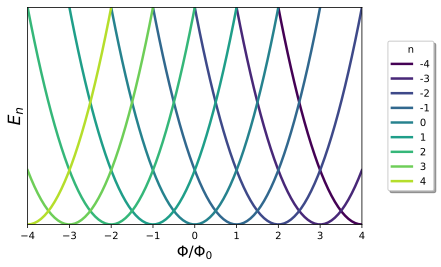
\includegraphics[width=\linewidth]{Immagini/topo/spectral_flow.pdf}
            \caption{Here plotted the energies $E_n$ (eq. \ref{spectral_flow} ), notice how the state \textit{"flow"} as we change $\Phi$}
        \end{figure}
    \subsection*{Parallelism with Bloch's Theorem}
    
        The keen eyed among you might have noticed that Figure 3 is suspicially similar to a crystal band structure in the limit on which the periodic potential $V\to 0$ with periodicity $2\pi$, let's see if this analogy holds \textit{the test of math}. Let's start by taking the single-particle free propagating Hamiltonian 
        \[
            H=\frac 1{2m}p_\theta^2
        \]
        The eigenstates this time have to respect the condition that $u_{n,q}(\theta)=e^{i2\pi q}u_{n,q}(\theta+2\pi)$.\footnote{This come from the block's theorem that states that the eigenstates of the hamiltonian of a periodic potential with periodicity $a$ mush obey that $u_{n,q}(x)=e^{iaq}u_{n,q}(x+a)$. In our case the periodicity $a=2\pi$ and the variable of the function is $\theta$ instead of $x$} This also means that if we substitute $q\to q+1$ the spectrum doesn't change. 
        % \begin{addmargin}[2em]{2em}
        %     \subsubsection*{Brief proof}
        %     A brief proof of this is the following:\\
        %     The problem of the eigenvalues can be written like so 
        %     \[
        %         He^{iq\theta}u_{n,q}(\theta)=E_n(q)e^{iq\theta}u_{n,q}(\theta)
        %     \]
        %     if we now send $q\to q+1$ the equation above becomes
        %     \[
        %         He^{iq\theta}e^{i\theta}u_{n,q+1}(\theta)=E_n(q+1)e^{iq\theta}e^{i\theta}u_{n,q+1}(\theta)
        %     \]
        %     The terms $u'_{n,q}(\theta)\equiv e^{i\theta}u_{n,q+1}(\theta)$ are also periodic $u'_{n,q}(\theta)=u'_{n,q}(\theta+2\pi)$. If we put it back into the equation above we get
        %     \[
        %         He^{iq\theta}u'_{n,q}(\theta)=E_n(q+1)e^{iq\theta}u'_{n,q}(\theta)
        %     \]
        %     That is completely equivalent to the equation at the start of this footnote, this means that the eigenvalues are periodic with periodicity 1\\
        % \end{addmargin}

        We now make the following unitary transformation to obtain a $q$-depentant Hamiltonian.
        \[
            H(q)=e^{-iq\theta}He^{iq\theta}=\frac 1{2m}\bigg (p_\theta + \frac {\hbar q}R \bigg)^2
        \]
        We can easly map this hamiltonian to the one in equation \ref{EMHamiltonian2} just by difining $\Phi$ such that $\hbar q= \frac {e\Phi}{2\pi}$. 
        \begin{equation} \label{blochA}
            H(\Phi)=\frac 1{2m}\bigg(p_\theta + \frac{e\Phi}{2\pi R}\bigg)^2
        \end{equation}
        Since before we said that the system doesn't change if we substitute $q\to q+1$, it means that now the system remains unchanged if we send $\Phi \to \Phi+\Phi_0$. This is exactly the result obtained in the previous page.
    
    
        And the tranformed eigenstates $\psi_{n,q}=e^{-iq\theta}u_{n,q}$ is just the cell-periodic part of the Bloch function. It satified the stricter periodic boundary condition
        \begin{equation} \label{blochboundraty}
            \psi_{n,q}(\theta)=\psi_{n,q}(\theta +2\pi)
        \end{equation}
        As you can see equations \ref{blochA}  and \ref{blochboundraty} create a system that is mathematically equivalent to the particle moving in a ring around a flux tube \cite{WeinbergBloch}.






    \subsection*{Conditions to have spectral flow}
        Up until now we looked spectral flow the case where the particle is freely propagating, let's see what happens when we add a periodic potential $V(\theta)=V(\theta+2\pi)$
        \[
            H=\frac 1{2m}p_\theta^2 + V(\theta)
        \]
        Now the spectrum is still periodic, however the energy bands don't necessarely cross, this means that  when abiabatically changing $q$, (or equivalently $\Phi$) the states won't flow, instead they will return to their original state
        \begin{figure}[h]
            \includegraphics[width=\linewidth]{Immagini/topo/grosso-flow.png}
            \caption{Pictorial representation of what happens when changing $q$}
        \end{figure}
        Conversely if there are $n$ degeneracies, on every cycle more the $i$-th stathe will flow to the $i+n$-th state


    
    \subsection*{Spectral flow in a more general context}
    
        The spectral flow is applicable in much more complex geometries than the one we have seen so far.\\
        Suppose that now the particle can moove in a 3D potential $V(\mathbf r)$, the Hamiltonian is
        \[
            H(\mathbf A)=\frac 1{2m}(\mathbf p + e\mathbf A)^2 + V(\mathbf r) 
        \]

        Since the solenoid is still the same, the formula for $\mathbf A$ remains unchanged (eq. \ref{vector_potential} )
        \[
            H(\Phi)=\frac 1{2m}\bigg(\mathbf p + \frac{e\Phi}{2\pi R}\hat \theta\bigg)^2 + V(\mathbf r)
        \]
        and since it's expressed in cylindrical coordinates it's better to express also $\mathbf p$ in cylindrical coordinates.
        \[
         \mathbf p =-i\hbar \mathbf \nabla=-i\hbar\bigg( 
             \mathbf{\hat r}\frac{\partial}{\partial r}+ \frac{\mathbf {\hat \theta}}{r}\frac{\partial}{\partial \theta} + \mathbf{\hat z}\frac{\partial}{\partial z}  \bigg) \equiv
             \mathbf{\hat r} p_r+ \mathbf {\hat \theta} p_\theta + \mathbf{\hat z} p_z
        \]
        Of course if we send $\theta \to \theta + 2\pi$ the system should be unchanged.
        \[
            \psi(r,\theta,z)=\psi(r,\theta+2\pi,z)
        \]
        Following the inverse reasoning done in the previous subsection we make the following unitary transformation.
        \[
            H=e^{i\theta\Phi/\Phi_0}H(\Phi)e^{-i\theta\Phi/\Phi_0}=\frac  {\mathbf p^2} {2m} + V(\mathbf r)
        \]
        This means that the eigenvalue probelm is now written like so
        \[
            He^{i\theta\Phi/\Phi_0}\psi(r,\theta,z)=E(\Phi)e^{i\theta\Phi/\Phi_0}\psi(r,\theta,z)
        \]

        If we send $\Phi \to \Phi+\Phi_0$ we get an equivalent equation
        \[
            He^{i\theta\Phi/\Phi_0}\psi(r,\theta,z)=E(\Phi+\Phi_0)e^{i\theta\Phi/\Phi_0}\psi(r,\theta,z)
        \]

        this means that the energy spectrum is unchanged if we send $\Phi \to \Phi+\Phi_0$. This is true regardless of the shape or geometry of $V(\mathbf r)$.
        
    
    \subsection*{The quantum Hall effect}

    
    
        We'll now see the effects of the spectral flow on physical properties of materials. Suppose we have a system like the one of the figure on the side. Now we slowly increase $\Phi$ from 0 to $\Phi_0$ in a total time $T$. This introduces a electromagnetice force arround the ring $\mathcal{E}=-\partial_t\Phi=-\Phi_0/T$.
    
    
        Let's suppose that the disc has the property that due to spectral flow $n$ electrons are transferred form the inner cirlce to the outer cicle in this time $T$. This would result in a radial current $I_r=-ne/T$. This means that the resistance is 
        \begin{equation} 
            \label{hall_resistivity}
                R_{xy}=\frac{\mathcal {E}}{I_r}=\frac{2\pi\hbar}{e^2}\frac 1n
        \end{equation}
        However, to be able to calculate $n$ we need to calculate how is the spectrum of the system as we change $\Phi$. This means that $n$ depends on the system, but equation \ref{hall_resistivity} is independent of the system. \footnote{There is the caveaut here that the system has to be in a defined quantum state, so in real world system it means that $T\approx0$}
	\chapter{Berry phase and Berry curvature}
\section{Introduction}
    Berry phase is the simplest demostration of how geometry and topology can emerge from quantum mechanics and it is in the heart of the quantum Hall effect\newline
    Let us consider a physical system described by a Hamiltonian that depends on a set of parameters $\boldsymbol \lambda=(\lambda_1,\lambda_2,\dots)$. These parameters do not represent the degrees of freedom of the system like position and momentum, rather they describe things such as the mass of a particle, the strenght of a potential and so on.\\ For each $H(\boldsymbol \lambda)$ there exists a set of eigenstates such that 
    \begin{equation}
        H(\boldsymbol \lambda)\ket{n,\boldsymbol \lambda}=E_n(\boldsymbol \lambda)\ket{n,\boldsymbol \lambda}
    \end{equation}
    However the equation above does not completely determine the basis function $\ket{n,\boldsymbol \lambda}$; We can change arbitrarly the phase $\gamma_n(\boldsymbol \lambda)$ of any eigenstate which is called \textit{Berry phase}
    \begin{equation}
        \label{eq:berryphase}
        \ket{n,\boldsymbol \lambda}\to \underbrace{e^{i\gamma_n(\boldsymbol \lambda (t))}}_{\textrm{Berry phase}} \ket{n,\boldsymbol \lambda}  
    \end{equation}
    Suppose we start off with a hamiltonian and than we slowly change the parameters for a time $T$ until it reaches a different hamiltonian, this means that $\boldsymbol \lambda=\boldsymbol \lambda(T)$. For the adiabatic theorem we can say that if we start on an energy eigenstate, and the system changes slowly enough
    \footnote{How slow you have to be in changing the parameters depens on the energy gap from the state you're in to the nearest other state. The smaller the gap, the slower you have to change the parameters. A way of showing this without doing long calculations is the following: \\ We know from the Heisemberg uncertanty principle that $T \Delta E \ge \hbar/2$. We want the uncertanty in the Energy to be way smaller than the energy gap$E_g \gg\Delta E$, so $E_g \gg \frac{\hbar}{2T}$, so if we make $T$ big enought it can be archieved},
    and has no degeneracies, then the system will cling on that energy eigenstate.\newline
    This means that the equation of motion of a particle that for time $t=0$ is equal to $\ket{\psi_n(t=0)}=\ket{n,\boldsymbol \lambda(0)}$ is 
    \begin{equation}
        \label{eq:psin}
        |\psi_n(t)\rangle=\underbrace{e^{i\gamma_n(\boldsymbol \lambda (t))}}_{\textrm{Berry phase}}\cdot
        \underbrace{e^{-\frac i\hbar\int_0^t E_n(\boldsymbol \lambda (t')) dt'}}_\textrm{dynamical phase}|n,\boldsymbol \lambda (t)\rangle      
    \end{equation}
    Where the first exponent comes from eq. \ref{eq:berryphase}. We now insert the equation above into the time-dependent Shrodinger equation
    \begin{equation}
        \label{eq:shrodt}
        i\hbar\partial_t|\psi_n(t)\rangle=H(\boldsymbol \lambda(t)) |\psi_n(t)\rangle
    \end{equation}
    By plugging equation \ref{eq:psin} into the \textit{right} term term of equation \ref{eq:shrodt} we get we get that
    \begin{equation}
        \label{eq:H(t)}
        H(\boldsymbol \lambda(t)) |\psi_n(t)\rangle = E_n(t)\ket{\psi_n(t)}
    \end{equation}
    Andy By plugging equation \ref{eq:psin} into the \textit{left} term term of equation \ref{eq:shrodt} we get we get that

    \begin{equation}
        \label{eq:psin-t}
        i\hbar\partial_t|\psi_n(t)\rangle=
        -\hbar \dot \gamma_n(t)|\psi_n(t)\rangle + E_n(t)|\psi_n(t)\rangle + e^{i\phi_n(t)}\partial_t|n,t\rangle
    \end{equation}
    where we have defined $e^{i\phi_n(t)} \equiv e^{i\gamma_n(\boldsymbol \lambda (t))}e^{-\frac i\hbar\int_0^t E_n(\boldsymbol \lambda (t')) dt'}$

    By equating the right terms in equations \ref{eq:H(t)} and \ref{eq:psin-t} we get that 
    \begin{equation}
        \label{eq:psin-t-H}
            i\hbar e^{i\phi_nt(t)}\partial_t|n,t\rangle=\hbar\dot \gamma_n(t)\ket{\psi_n(t)} =\hbar\dot \gamma_n(t)e^{i\phi_n(t)}\ket{n,t}
    \end{equation}    
    now we multiply the term on the left and on the right of equation \ref{eq:psin-t-H} by $\hbar^{-1}e^{-i\phi_n(t)} \bra{n,t}$
    \begin{equation}
        \label{eq:psin-t-H-bra}
            \dot \gamma_n(t)=i\bra{n,t} \partial_t\ket{n,t}
    \end{equation}
    We can re-express it in terms of $\boldsymbol \lambda$
    \begin{equation}
        \label{eq:connection}
            \dot \gamma_n(t)=\dot{\boldsymbol \lambda}\cdot\underbrace{i\bra{n,t} \partial_{\boldsymbol \lambda}\ket{n,t}}_{\equiv \mathbf A_n(\boldsymbol \lambda)}
    \end{equation}
    Where $\mathbf A_n(\boldsymbol \lambda)$ called the \textbf{Berry connection}
    This means that we can calculate the total change in $\gamma_n(t)$ can be obtained by doing a line integral in the space of parameters $\boldsymbol \lambda$ over the path $\mathcal P$ of values that $\boldsymbol \lambda$ assumes during the time evolution

    \begin{equation}
        \label{eq:line_int1}
            \gamma_n=\int_\mathcal{P} \mathbf A_n(\boldsymbol \lambda) \cdot d\boldsymbol \lambda
    \end{equation}


    \begin{equation}
        \label{eq:re-define}
        \ket{n,\boldsymbol \lambda}\to e^{if_n(\boldsymbol \lambda)}\ket{n,\boldsymbol \lambda}
    \end{equation}

    Keep in mind however that the eigenstates are defined up to a phase, meaning that we can re-define the base vectors like so 
    (equation \ref{eq:re-define}). If we apply this substitution
    into the formula of $\mathbf A_n$ we have that

    \[
    \mathbf A_n(\boldsymbol \lambda) =i\bra{n,t} \partial_{\boldsymbol \lambda}\ket{n,t}\to i\bra{n,t} \partial_{\boldsymbol \lambda}\ket{n,t} - \partial_{\boldsymbol \lambda}f_n(\boldsymbol \lambda)
    \]

    \begin{equation}
        \label{eq:gauge1}
        \mathbf A_n \to \mathbf A_n - \partial_{\boldsymbol \lambda}f_n
    \end{equation}
        So the system is invariant under the gauge transformation in equation \ref{eq:gauge1}.  If we do this transformation to equation \ref{eq:line_int1} we have that

    \[
        \gamma_n=\int_\mathcal{P} \mathbf A_n(\boldsymbol \lambda) \cdot d\boldsymbol \lambda - \int_\mathcal{P} \partial_{\boldsymbol \lambda}f_n(\boldsymbol \lambda) \cdot d\boldsymbol \lambda= \int_\mathcal{P} \mathbf A_n(\boldsymbol \lambda) \cdot d\boldsymbol \lambda + f(\boldsymbol \lambda(0))-f(\boldsymbol \lambda (T))
    \]
    This means that if the path $\mathcal{P}$ is open we can always choose a function $f_n$ such that 
    $f(\boldsymbol \lambda(0))-f(\boldsymbol \lambda(T))=\int_\mathcal{P} \mathbf A_n(\boldsymbol \lambda) \cdot d\boldsymbol \lambda$, 
    thus we can conclude that one can always choose a suitable $f(\boldsymbol \lambda)$ such that $\gamma_n$ accumulated along the path $\mathcal P$ is calceled out leaving equation 
    \ref{eq:psin} with only the dynamical phase. 
    However if the path is closed $\boldsymbol \lambda(0)=\boldsymbol \lambda(T)$, in order to make the phase change
    in equation \ref{eq:re-define} single value we must have that
    \[
    e^{f(\boldsymbol \lambda(0))-f(\boldsymbol \lambda(T))}=1
    \]
    so 
    \[
        f(\boldsymbol \lambda(0))-f(\boldsymbol \lambda(T))=2n\pi \quad n\in \mathbb{R}
    \]
    This leads us to the important result that
    \begin{equation}
        \label{eq:closed-berry}
        \gamma_n=\oint_{\mathcal P} \mathbf A_n(\boldsymbol \lambda)\cdot d\boldsymbol \lambda + 2n\pi
    \end{equation}
    This time, if the line integral is not a multiple of $2\pi$ (and there is no reason why it should) there is no way of choosing a suitable $f_n$ to
    cancel it out and the Berry phase in equation \ref{eq:psin} is there to stay



\section{Berry curvature}
    In EM the field thensor $F_{\mu\nu}$ is defined as in equation \ref{eq:EM-field-tensor}.
    Since Berry conenction has the same Gauge invariance as the one of the EM vector potential it is useful to define, a gauge field tensor derived from the Berry connection:
    \begin{equation}
        \label{eq:EM-field-tensor}
        F_{\mu\nu}=\partial_\mu A_\nu-\partial_\nu A_\mu
    \end{equation}

    \begin{equation}
        \label{eq:berry-curvature1}
            \Omega_{\mu\nu}^n =\partial_\mu A^n_\nu(\boldsymbol \lambda) - \partial_\nu A^n_\mu(\boldsymbol \lambda)
    \end{equation}
    This new field tensor is defined as \textbf{Berry curvature} and it is gauge independent just like 
    $F_{\mu\nu}$!\footnote{The notation has changed a bit, now $A_\mu^n\equiv (\mathbf A_n)_\mu$}

    \subsection{Other formulas for $\Omega_{\mu\nu}$}

        With a few mathematical steps it is possible to re cast the Berry curvature into a different form that might be useful later
        \[
            \partial_\mu A^n_\mu =i\partial_\mu \bra{n,\boldsymbol \lambda}\partial_\nu n,\boldsymbol \lambda \rangle= 
            i\bra{\partial_\mu n,\boldsymbol \lambda}\partial_\nu n,\boldsymbol \lambda \rangle + i\bra{n,\boldsymbol \lambda}\partial_\mu\partial_\nu n,\boldsymbol \lambda \rangle
        \]
        \begin{equation}
            \label{eq:berry-curvature2}
                \boxed{\Omega_{\mu\nu}^n =i\bra{\partial_\mu n}\partial_\nu n\rangle - i\bra{\partial_\nu n}\partial_\mu n\rangle}
        \end{equation}


        It is also possible to express $\Omega$ in terms of the eigenstates of the Hamiltonian with some mathematical manipulation
        \[
            \bra{n'} H \ket{n}=\delta_{n'n} \to \partial_\mu \bra{n'} H \ket{n}=0
        \]
        \[
        \partial_\mu \bra{n'} H \ket{n}=\bra{\partial_\mu n'}H\ket{n} + \bra{n'}H\ket{\partial_\mu n} + \bra{n'} \partial_\mu H\ket{n}
        \]
        \[
            E_{n}\bra{\partial_\mu n'}n\rangle + E_{n'} \bra{n'}\partial_\mu n\rangle=\bra{n'} \partial_\mu H\ket{n}
        \]
        \[
            (E_{n'}-E_n)\bra{n'} \partial_\mu n\rangle=\bra{n'} \partial_\mu H\ket{n}
        \]
        \begin{equation}
            \label{eq:partial H}
                \bra{n'}\partial_\mu n\rangle=  \frac{\bra{n'} \partial_\mu H\ket{n}}{E_{n'}-E_n}
        \end{equation}

        Now we write equation \ref{eq:berry-curvature2} like so
        \[
            \Omega_{\mu\nu}^n =i\bra{\partial_\mu n}\partial_\nu n\rangle - (\mu \leftrightarrow \nu)= i\sum_{n'\neq n}\bra{\partial_\mu n}n'\rangle\bra{n'}\partial_\nu n\rangle - (\mu \leftrightarrow \nu)
        \]
        By plugging in above equation \ref{eq:partial H} we get
        \begin{equation}
            \label{eq:berry-curvature3}
            \boxed{\Omega_{\mu\nu}^n=i\sum_{n'\neq n} \frac{\bra{n}\partial_\mu H\ket{n'}\bra{n'} \partial_\nu H\ket{n}}{(E_{n'}-E_n)^2}- (\mu \leftrightarrow \nu)}
        \end{equation}
        This last form of the Berry curvature has the advantage that no differentiation of the wavefunction is needed. This equation also tells us that
        \[ \sum_n \Omega_{\mu\nu}^n (\boldsymbol \lambda)=0 \]


    \section{Stokes' Theorem}
    \begin{figure}
        \centering
        \includegraphics[width=0.7\linewidth]{Immagini/stokes.eps}
        \caption{Here we divide the surface of the sphere in two different surfaces $\mathcal A$ and $\mathcal B$ that share the edge $\mathcal P$}
    \end{figure}
    From the Stokes theorem we have that
    \begin{equation}
        \label{eq:stokes}
            \gamma_n=\oint_\mathcal{P} A^n_\mu\: d\lambda^\mu=\frac 12 \int_\Sigma \Omega_{\mu\nu}^n\: d\lambda^\mu \wedge d\lambda^\nu
    \end{equation}
    where we have used the Einstein convention of summation and the $\wedge$ operator represents the exterior product\newline
    There is a subtelty in this last equation, as we know the Berry curvature tensor in Gauge-invariant, so the integral over the surface is too, but the integral over the closed path of the Berry connection is defined up to a factor $2n\pi$ that is gauge dependant.
    So is there a modulo $2\pi$ ambiguity or not?\newline
    The answer is that if $\gamma_n$ is to be determined using the knowledge of $\ket{n,\boldsymbol \lambda}$ 
    only on the curve $\mathcal P$ then it is really well defined modulo $2\pi$. In this case we can re-write 
    equation \ref{eq:stokes} as 
    \[
    \frac 12 \int_\Sigma \Omega_{\mu\nu}^n\: d\lambda^\mu \wedge d\lambda^\nu:=\oint_\mathcal{P} A^n_\mu\: d\lambda^\mu
    \]
    Meaning that the integral over the surface $\mathcal \Sigma$ is equal to \textit{one of the values of} the integrals along the closed path $\mathcal P$\newline

    But what kind of Gauge gives the "correct" answer? If we choose a gauge that is continuous and smooth
    everywhere along the surface $\Sigma$ including on its boundary $\mathcal P$ then equation \ref{eq:stokes} becomes unambiguous.\newline
    While it is possible to make a radical gauge transformation that shifts $\gamma_n$ by $2\pi$ when regarding $\ket{n,\boldsymbol \lambda}$ as a function defined only in the neighborhood of $\mathcal P$, such a gauge change cannot be smoothly continued into the interior $\mathcal S$ without creating a vortex-like singularity of $\gamma_n(\boldsymbol \lambda)$.


\section{Chern Theorem}
    
    Let's take as an example Gauss's theorem. It tells us that the flux of the field through a closed surface is equal to the charges inside. \newline
    Now let's calculate the flux of the Berry curvature thorugh a closed surface. We can divide the closed surface as two different open surfaces that share the same edge $\mathcal P$.\newline
    Thanks to stokes theorem the flux throught the surface $\mathcal A$ is $\oint_\mathcal{P} \mathbf A \cdot d\boldsymbol \lambda$, but the flux throught the surface $\mathcal B$ is $-\oint_\mathcal{P} \mathbf A \cdot d\boldsymbol \lambda$.\newline
    Theese two integrals must be equal modulo $2\pi$, so
    \begin{figure}
        \centering
        \includegraphics[width=0.85\linewidth]{../website/images/berry/chern_theorem.png}
        \caption{Here we divide the surface of the sphere in two different surfaces $\mathcal A$ and $\mathcal B$ that share the edge $\mathcal P$}
        \label{fig:forward_pass}
    \end{figure}
    \begin{equation}
        \label{eq:chern}
        \oint_\mathcal{S} \Omega_{\mu\nu}^n d\lambda^\mu \wedge d\lambda^\nu =2\pi C \quad\quad C\in \mathbb Z
    \end{equation}
    This means that the flux thought a closed surface of the Berry curvature is quantized
    
    The constant $C$ in known as the Chern number. Note that when the Chern index is nonzero, it is impossible to construct a smooth and continuous gauge over the entire surface $\mathcal{S}$. If such a gauge did exist, then we could apply Stokes’ theorem directly to the entire surface and conclude that the Chern number vanishes, in contradiction with the assumpti\newline
    But what are theese "pseudo-charges" inside the closed surface that generate the flux?\newline
    In E.M. a simple way to spot charges (or monopoles) is to look at the field tensor and see if as some point it diverges as $1/(\mathbf r-\mathbf{r_0})^2$. Let's take a look at $\Omega_{\mu\nu}$ (eq. \ref{eq:berry-curvature3}) and see if we can spot anything similar \footnote{In the equation below I expressed explicitely the $\boldsymbol \lambda$ dependence in the denomiator and condensed the fomula using the wedge product $\wedge$}
    \begin{equation}
        \label{eq:monopoles1}
        \Omega_{\mu\nu}^n=i\sum_{n'\neq n} \frac{\bra{n}\partial_\mu H\ket{n'}\wedge \bra{n'} \partial_\nu H\ket{n}}
        {\underbrace{[E_{n'}(\boldsymbol \lambda)-E_n(\boldsymbol \lambda)]^2}_
        {\substack{\text{what happens if for some } \boldsymbol \lambda=\boldsymbol \lambda_d  \\\text{ the two energies are the same?}}}}
    \end{equation}

    So, suppose that for some $\boldsymbol \lambda=\boldsymbol \lambda_d$ we have that $E_n (\boldsymbol \lambda_d)=E_m(\boldsymbol \lambda_d)$, now we expand the energies near $\boldsymbol \lambda_d$ at first order
    \[
    \begin{cases}
    E_n(\boldsymbol \lambda)\, \approx E_n(\boldsymbol \lambda_d) +\, \partial_{\boldsymbol \lambda} E_n|_{\boldsymbol \lambda =\boldsymbol \lambda_d}\cdot (\boldsymbol \lambda-\boldsymbol \lambda_d)\\
    E_m(\boldsymbol \lambda)\approx E_n(\boldsymbol \lambda_d) + \partial_{\boldsymbol \lambda} E_m|_{\boldsymbol \lambda =\boldsymbol \lambda_d}\cdot (\boldsymbol \lambda-\boldsymbol \lambda_d)\\

    \end{cases}
    \]
    This means that 
    \[
    E_n(\boldsymbol \lambda)-E_m(\boldsymbol \lambda)\approx \partial_{\boldsymbol \lambda} (E_n-E_m)|_{\boldsymbol \lambda =\boldsymbol \lambda_d}\cdot (\boldsymbol \lambda-\boldsymbol \lambda_d)
    \]
    so the denominator of the berry curvature near $\boldsymbol \lambda_d$ goes like $ 1/(\boldsymbol \lambda-\boldsymbol \lambda_d)^2$.\newline
    This means that there are "charges" or "monopoles" that induce the flux throught the closed surface, and they are localized where 2 (or more) energy levels cross

	%%\chapter{Spin-polarized drift-diffusion}
	\section{Kubo Formula}
We'll derive the Kubo formula for a general, multi-particle (or, if you prefer, single particle) Hamiltonian $H_0$ where the subscript 0 means that this is the unperturbed Hamiltonian before we apply an electric field. We denote the eigentstates of the Hamiltonian as $\ket m$ with $H_0\ket m=E_m \ket m$.
\begin{equation}
    H_0=\sum_i\left[\frac{1}{2m}\left(\vect p_i-e\vect A_0\right)^2 + V_0(\vect r_i)\right]+\sum_{i\neq j}V_{ee}(\vect r_i-\vect r_j)
\end{equation}
Where $\vect A_0$ and $V_0$ are due to an existing EM field. Now we add a background electric field. We 
\begin{equation}
    H=\sum_i\left[\frac{1}{2m}\left(\vect p_i-e\vect A_0 - e\vect A\right)^2 + V_0(\vect r_i) - e\vect r_i\phi(\vect r_i)\right]+\sum_{i\neq j}V_{ee}(\vect r_i-\vect r_j)
\end{equation}
Which can be written as 
\begin{equation}
    H=H_0 + \sum_{i}-\frac{e}m \boldsymbol \pi_i\cdot \vect A - e\vect r_i\phi(\vect r_i)
    \label{eq:temp_ham}
\end{equation}
Where $\boldsymbol \pi_i=\vect p -e\vect A_0=m\dot{\vect r}$ is the mechanical momentum,
furthermore we can use the fact that the electric charge operator $\rho(\vect r)=-e\sum_{i}\delta(\vect r-\vect r_i)$ current operator  $\vect J$ is equal to 
\begin{equation}
    \vect J=-e\sum_{i}\dot{\vect r}_i=-\sum_{i}\frac{e}m \boldsymbol \pi_i
\end{equation}
to re-write equation \ref{eq:temp_ham} like so
\begin{equation}
    H=H_0+\vect J\cdot \vect A + \int\rho(\vect r)\phi(\vect r)d\vect r
\end{equation}
however, we can assume that the density of charge $\rho$ is always zero
\begin{equation}
    H=H_0+\vect J\cdot \vect A
\end{equation}
At this point we need to write the perturbation in terms of the electric field, we can choose a gauge where $\vect E=-\partial_t\vect A$ and assume that the wave is monochromatic $\vect E(t)=\vect Ee^{-i\omega t}$, so 
\begin{equation}
    A=\frac{ \vect E}{i\omega}e^{i\omega t}
\end{equation}
	\chapter{Introduction to relevant topics}
Graphene is a two-dimensional lattice of carbon atoms, arranged in a honeycomb structure as shown in the figure \ref{fig:graphene} Although it is straightforward to build many layers of these lattices (a substance known as graphite), it was long thought that a purely two-dimensional lattice would be unstable to thermal fluctuations and impossible to create.
This changed in 2004 when Andre Geim and Konstantin Novoselov succeeded in isolating two-dimensional graphene \cite{firstExfoliation}. For this, they won the 2010 Nobel prize. As we now show, the band structure of graphene is particularly interesting.
\begin{figure}[h]
    \makebox[\textwidth][c]{
        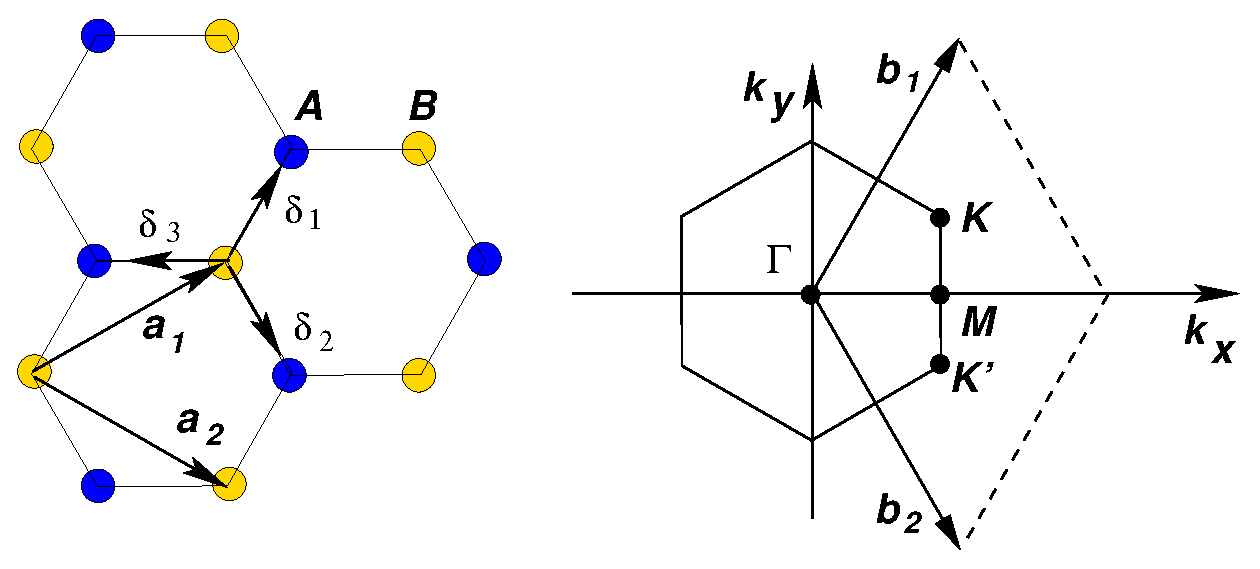
\includegraphics[width=\linewidth]{Immagini/graphene/structure.eps}
        }%
    \caption{On the left there is the lattice structure of graphene made out of two interpenetrating triangular lattices ($a_1$ and $a_2$ are the lattice unit vectors, and $\mathbf \delta_{i}$ with $i\in {1,2,3}$ are the nearest neighbors. On the right the corresponding Brillouin zone, the Dirac cones are located at the $K_0$ and $K_1$ points) \cite{guinea2008review}}
    \label{fig:graphene}
\end{figure}\\
We define the primitive lattice vectors $\vect a_1$ and $\vect a_2$ as follows:
\begin{equation}
    \vect a_1=\frac{a}2
    \begin{bmatrix}
        3 \\ \sqrt 3
    \end{bmatrix}\quad \quad
    \vect a_2=\frac{a}2
    \begin{bmatrix}
        3 \\ -\sqrt 3
    \end{bmatrix}
\end{equation}
Where $a$ is the distance between two neighboring atoms, which in graphene is $\approx 1.4\times 10^{-10}$m. The sublattice A is defined as all the points $r = n_1\vect a_1 + n_2\vect a_2$ with $n_i \in \mathbb Z$ (yellow in figure \ref{fig:graphene}), sublattice B is defined as all points $r = n_1\vect a_1 + n_2\vect a_2 + \delta$ with $\delta = (a, 0)$ (blue in figure \ref{fig:graphene}). These are the white dots.

The reciprocal lattice vectors $\vect b_i$ are the vectors that satisfy $\vect a_i\cdot \vect b_j=\delta_{ij}$ and are equal to 
\begin{equation}
    \vect b_1=\frac{2\pi}{3a}\begin{bmatrix}
        1 \\ \sqrt 3
    \end{bmatrix}
    \quad \quad
    \vect b_2=\frac{2\pi}{3a}\begin{bmatrix}
        1 \\ -\sqrt 3
    \end{bmatrix}
\end{equation}
This reciprocal lattice is also triangular. The Brillouin zone is constructed in the usual manner by drawing perpendicular boundaries between the origin and each other point in the reciprocal lattice giving rise to a hexagonal Brillouin zone with $K_0$ and $K_1$ as the vertices of the hexagon, where 
\[
    K_0=\frac 13 (2b_1+b_2)\quad \quad K_1=\frac 13 (b_1+2b_2)
\]

\begin{equation}
    K_0=\frac{2\pi}{3a}\left(1,\frac 1{\sqrt 3}\right)\quad\quad K_1=\frac{2\pi}{3a}\left(1,-\frac 1{\sqrt 3}\right)
\end{equation}

\subsubsection*{The tight binding approach}
To investigate the band structure of graphene, we are going to use the tight binding approach \cite{bloch1929quantenmechanik}.
First we write the Hamiltonian.
\begin{equation}
    H=\frac{\vect p^2}{2m} + \sum_{\vect R\in C}V(x-\vect R)
    \label{eq:blochhamiltonian}
\end{equation}
where the set $C=\left\{n_1\vect a_1 +n_2\vect a_2 + j\boldsymbol \delta\,|\,n_1,n_2\in \mathbb Z,\, j\in \{0,1\} \right\}$ is the set of all the positions of the atoms.

Let $\ket{n,\vect R}$ be the $n$-th eingenstate of the Hamiltonian of a carbon atom placed in $\vect R$.
Due to translational symmetry, the wave function must satisfy the Bloch theorem, this tells us that the eingenstates of the Hamiltonian can be written as
\begin{equation}
    \ket{n,\vect k}=\sum_{\vect R\in C} e^{i\vect k \cdot \vect R}\ket{n,\vect R}
\end{equation}
With this we can now calculate the matrix elements of the Hamiltonian
\begin{equation}
    \big\langle n,\vect k\big|H\big| n',\vect k'\big\rangle=
    \sum_{\vect k\vect k',\vect R\vect R'}e^{i\vect k\cdot \vect R-i\vect k'\cdot\vect R'}
    \big\langle n,\vect R\big|H\ket{n',\vect R'}
\end{equation}
Since the right-hand side of the summation does not depend on $k$ we have that the terms with $k\neq k'$ are equal to zero. So the equation above becomes
\[
    \big\langle n,\vect k\big|H\big| n',\vect k'\big\rangle= \big\langle n,\vect k\big|H\big| n',\vect k\big\rangle\delta_{\vect k,\vect k'}
\]
Ok, now we need to calculate $ \big\langle n,\vect R\big|H\ket{n',\vect R'}$. Using equation \ref{eq:blochhamiltonian} we get that if $\vect R=\vect R'$
\begin{equation}
    \big\langle n,\vect R\big|H\ket{n',\vect R}=E_n\delta_{n,n'}+
    \underbrace{
        \sum_{\vect R'\neq \vect R}
        \big\langle n,\vect R\big|V(r-\vect R')\ket{n',\vect R}
    }_{\text{small}}
    \label{eq:tight1}
\end{equation}
The second term is much smaller than the first one, so we can ignore it.\\
In the case where $\vect R$ and $\vect R'$ are two nearest neighbors we have that $\vect R'=\vect R+\boldsymbol\delta_i$ with $i\in \{1,2,3\}$ (fig. \ref{fig:graphene}).\\ We can expand the state localized in $\vect R'$ in terms of the ones localized in $\vect R$

\begin{equation}
    \ket{n',\vect R +\boldsymbol\delta_i}=
    \sum_{n''}\ket{n'',\vect R}\braket{n'',\vect R}{n',\vect R+\boldsymbol\delta_i}=
    \sum_{n''}\ket{n'',\vect R}t_{nn'}^1
\end{equation}
Where $t_{nn'}\equiv\braket{n,0}{n',\boldsymbol\delta_i}$
This means that 
\begin{equation}
    \big\langle n,\vect R\big|H\ket{n',\vect R'}=
    \sum_{n''}\bra{n,\vect R}H\ket{n'',\vect R}t_{n'n''}\approx
    E_n t_{nn'}^1
\end{equation}
where in the last step we used \ref{eq:tight1}

	\section{Gapped Graphene}
If either the sublattice symmetry $\mathcal P$ or the time reversal symmetry $\mathcal T$ are broken the Hamiltonian near the $\vect K$ points becomes a massive Dirac Hamiltonian.
This means that for materials that don't have the parity symmetry $\mathcal P$ such as Boron Nitrite exhibit an open gap in the $\vect K$ points, alternatively one could layer graphene on top of another honeycomb lattice that doesn't have sublattice symmetry, therefore subjecting it with a periodic potential that breaks the symmetry and opens the gap by adding a mass term $\Delta$ in both the Dirac cones.\\
Finding a crystalline structure that breaks time reversal symmetry can be a little more cumbersome, these kind of structures had been theorized by Haldane in 1987 \cite{haldane1988model}, then Kane and Mele \cite{kane2005quantum} proved that this happens in graphene itself if we take into account spin-orbit coupling, 


Mathematically speaking, the tight binding Hamiltonian has two different energies for the two different atoms in the sub-lattice. With respect to equation \ref{eq:dirac_Hamiltonian} it becomes
\begin{equation}
    H_{\vect K_0}(\vect k)=
    -H^*_{\vect K_1}(\vect k)=
    \begin{bmatrix}
        \Delta& v_F\hbar(k_x-ik_y)\\
        v_F\hbar(k_x+ik_y)&-\Delta
    \end{bmatrix}
    \label{eq:gapped-dirac}
\end{equation}
Where $\Delta$ is half the difference of the diagonal energy on the two sublattices, and the energy zero has been shifted at the center of the energy gap. The dispersion relation now becomes
\begin{equation}
    E(\vect k)=\pm\sqrt{\Delta^2 + (v_F\hbar k)^2}
\end{equation}
It is seen that the above dispersion curves are formally the same produced by the Dira equations, with the light velocity $c$ replaced by the Fermi velocity $v_F$ and the rest mass $m_0=\Delta/v_F^2$

\begin{figure}[h]
    \makebox[\textwidth][c]{
        \includegraphics[width=\linewidth]{Immagini/graphene/dirac.pdf}
        }%
    \caption{difference between the gapless and the gapped Dirac dispersion relation}
    \label{fig:dispersion-1D}
\end{figure}
	\section{Bilayer graphene}

In the tight-binding description of bilayer graphene, we take into account $2p_z$ orbitals on the four atomic sites in the unit cell, labelled as $j = A_1, B_1, A_2, B_2$. Then, the transfer integral matrix of bilayer graphene is a $4\times 4$  matrix given by \cite{McCann_2013}

\begin{equation}
    H(\vect k)=
    \begin{bmatrix}
        E_{A_1} & -\gamma_0 F(\vect k) & \gamma_4 F(\vect k) & -\gamma_3 F(\vect k)\\
        -\gamma_0 F(\vect k) & E_{B_1} & -\gamma_1 & \gamma_4 F(\vect k)\\
        \gamma_4 F(\vect k) & \gamma_1 & E_{A_2} & -\gamma_0 F(\vect k)\\
        -\gamma_3 F(\vect k)& \gamma_4 F(\vect k)& -\gamma_0 F(\vect k) & E_{B_2}
    \end{bmatrix}
\end{equation}

% 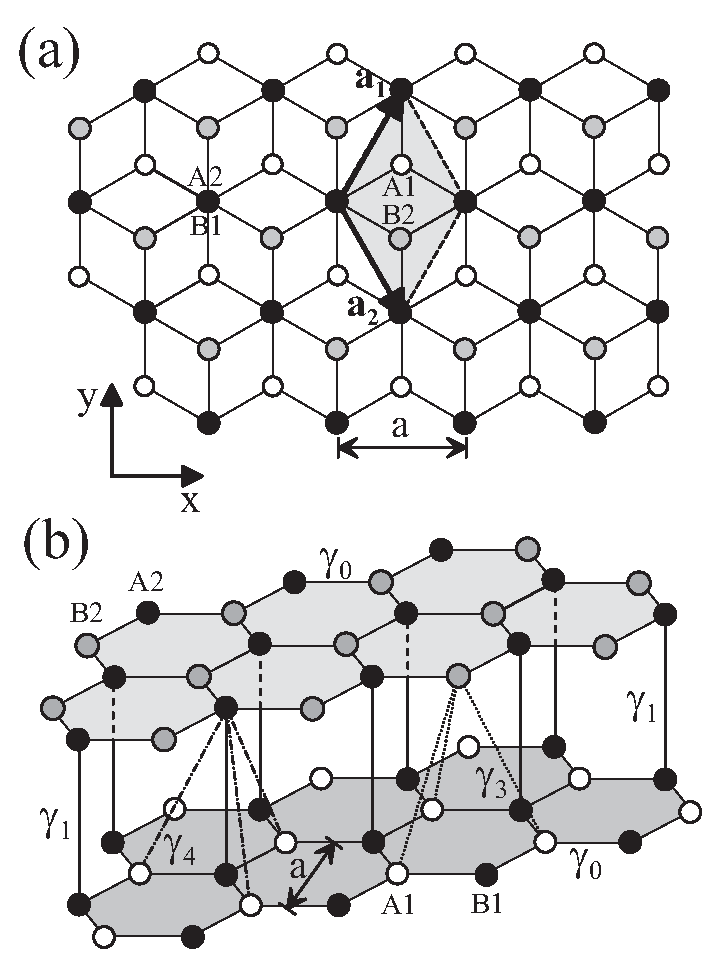
\includegraphics[width=\linewidth]{Immagini/graphene/bilayerlattice.eps}
% \caption{difference between the gapless and the gapped Dirac dispersion relation}
% \label{fig:bilayer-lattice}

\begin{table}[ht]
    \begin{minipage}[b]{0.56\linewidth}
    \centering
    \begin{tabular}{ l l r }
        \hline
        Parameter & Value [eV] \\ 
        \hline \hline
        $\gamma_0$ & $3.16\pm0.03$ \\
        $\gamma_1$ & $0.381\pm 0.003$ \\
        $\gamma_3$ & $0.38\pm 0.06$ \\
        $\gamma_4$ & $0.14\pm 0.03$ \\
        $s_0$ & boh\\
        $s_1$ & boh\\
        \hline
       \end{tabular}
        \caption{Values in eV of $\gamma_i$}
        \label{table:valuetable}
    \end{minipage}\hfill
    \begin{minipage}[b]{0.4\linewidth}
    \centering
    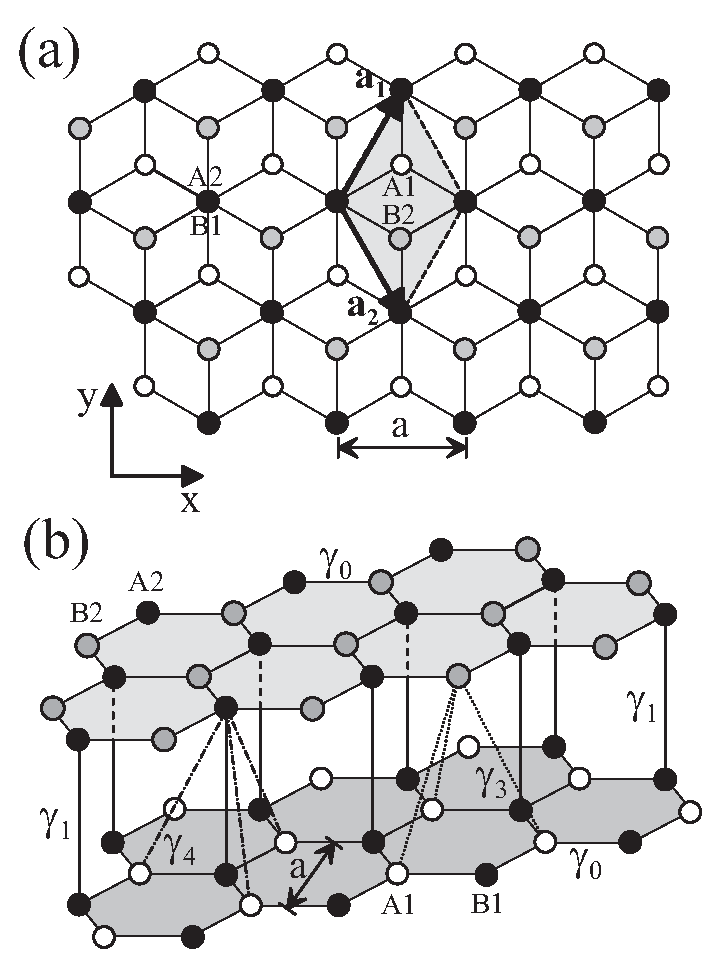
\includegraphics[width=\linewidth]{Immagini/graphene/bilayerlattice.eps}
    \captionof{figure}{Schematic representation of the bilayer graphene structure}
    \label{fig:bilayer-lattice}
    \end{minipage}
\end{table}

where the tight-binding parameters are defined as 
\begin{equation}
    \begin{split}
        \gamma_0=&-\braket{A_1|H}{B_1}=-\braket{A_2|H}{B_2} \\
        \gamma_1=&\braket{A_2|H}{B_1}  \\
        \gamma_3=&-\braket{A_1|H}{B_2}  \\
        \gamma_4=& \braket{A_1|H}{A_2}=\braket{B_1|H}{B_2} \\
    \end{split}
\end{equation}
The upper-right and lower-left square $2\times 2$ blocks of $H$ describe inter-layer coupling. Parameter $\gamma_1$ describes coupling between pairs of orbitals on sites that are directly above each other $B_1$ and $A_2$ (also called dimer sites): since this is a vertical coupling, the corresponding terms in $H$ do not contain $F(\vect k)$ which describes in-plane hopping. The other $\gamma$ factors do have an in plane component, which causes the $F(\vect k)$ term to show up.\\
The overlap matrix $S$ form equation $\ref{eq:overlap}$ becomes in the bilayer case
\begin{equation}
    S=
    \begin{bmatrix}
        1 & s_0 F(\vect k) & 0&0\\
        s_0 F(\vect k)  &1&s_1&0\\
        0&s_1&1&s_0 F(\vect k)\\
        0&0&s_0 F(\vect k) &1
    \end{bmatrix}
\end{equation}
Here we only include two parameters: $s_0 = \braket{A_1}{B_1} = \braket{A_2}{B_2}$ describing non-orthogonality of intra-layer nearest-neighbours and $s_1= \braket{A_2}{B_1}$ describing non-orthogonality of orbitals on dimer sites A1 and B2. In principle, it is possible to introduce additional parameters analogous to $\gamma_3,\gamma_4$, etc., but generally they will be small and irrelevant, infact in the bilayer case it is common practice to neglect completely the overlap matrix if we are dealing with. The resulting energy bands are plotted in figure \ref{fig:dispersion-bilayer}

\begin{figure}[h]
    \makebox[\textwidth][c]{
        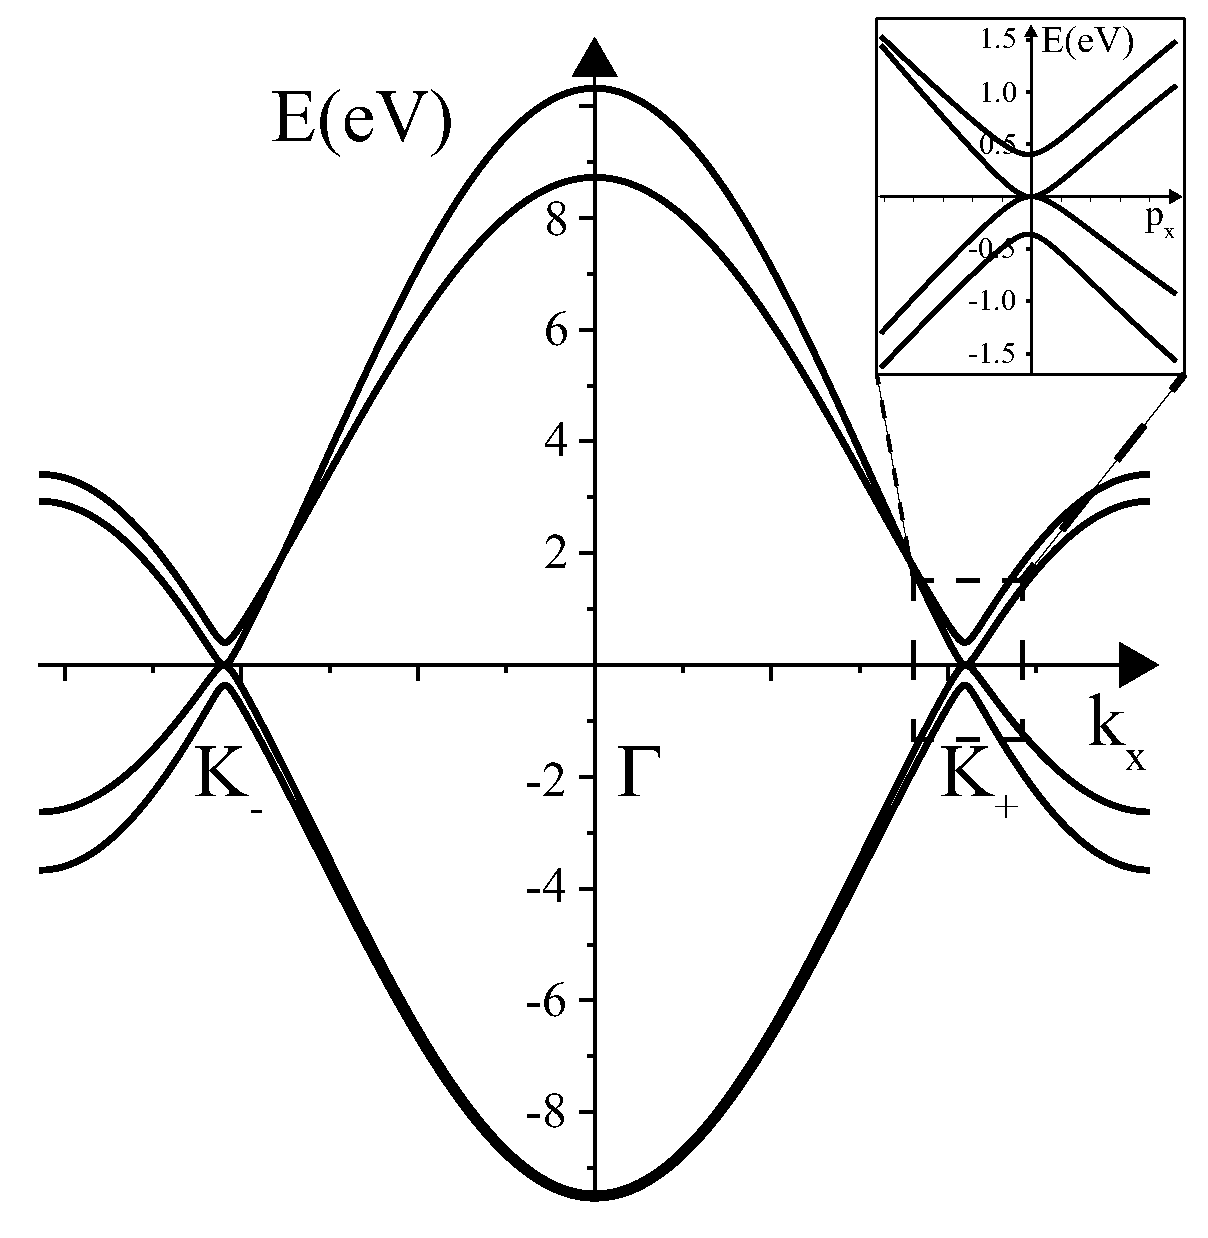
\includegraphics[width=.7\linewidth]{Immagini/graphene/bilayer-bands.eps}
        }%
    \caption{Here are plotted the $p_z$ orbitals along the $k_x$ axis in the reciprocal space intersecting the corners $K_0$ and $K_1$ and the center $\Gamma$ of the Brillouin zone. Notice how now we have four bands, this because we have four atoms in the fundamental cell, two for each layer}
    \label{fig:dispersion-bilayer}
\end{figure}
To describe the properties of the electrons near the $K$ we just have to approximate $F(\vect k)$ just like we did in equation \ref{eq:F(k)-approx}. This results in a Hamiltonian that is the generalization of the one we had in equation \ref{eq:gapped-dirac}

\begin{equation}
    H_{\vect K_0}=-H_{\vect K_1}^*=
    \begin{bmatrix}
        E_{A_1} & v_F\pi^\dag & -v_4\pi^\dag & v_3\pi\\
        v_F\pi& E_{B_1} & \gamma_1 & -v_4\pi^\dag\\
        -v_4\pi & \gamma_1 & E_{A_2} & v_F\pi^\dag\\
        v_3\pi^\dag & -v_4\pi & v_F\pi & E_{B_2}
    \end{bmatrix}
\end{equation}
Where $\pi= \hbar (k_x+ik_y),\pi^\dag=\hbar (k_x-ik_y)$, and the velocities $v_{3,4}=a\gamma_{3,4}/\hbar$ are effective fermi velocities that come from the coupling $\gamma_3$ and $\gamma_4$ CONTROLLA SE LA CONVERSIONE DELLA A è CORRETTA\\
A simple analytic solution may be obtained by neglecting the terms $v_4\pi$, $v_4\pi^\dag$ proportional to $\gamma_4$, and by considering only interlayer asymmetry $U$ in the on-site energies: $E_{A_1}=E_{B_1} = -U/2$ and $E_{A_2} = E_{B_2} = U/2$. Then, there is electron-hole symmetry, i.e., energies may be written $E = \pm E\alpha(\vect p), \alpha \in {1, 2}$

\begin{equation}
    \begin{split}
    &E_\alpha^2(\vect p)=\frac{ \gamma_1^2}2 + \frac{U^2}4+
    p^2\left(
        v^2+\frac{v^2_3}2
    \right)
    +(-1)^\alpha\,\sqrt{\Gamma}
    \\
    &\Gamma=\frac 14\left( \gamma_1^2-v_3^2p^2\right)^2+
    v^2p^2\left(\gamma_1^2+U^2+v_3^2p^2 \right)+ 
    2\zeta\gamma_1v_3v^2\cos(3\theta)
    \end{split}
\end{equation}
were $\theta$ is the polar angle of the impulse $\vect k=(k_x,k_y)=k(\cos\theta,\sin\theta)$


	\chapter{Anomalous Hall effect}
	The anomalous Hall effect refers to the appearance of a large spontaneous Hall current in ferromagnet in response to an electric field alone \cite{vanderbilt2018berry}, and it was first discovered by Hall in 1881 \cite{hall1881}. Despite its century long history and importance, the microscopic characterization of the anomalous Hall effect has been a controversial subject. In the past three main mechanisms have been identified:
\begin{itemize}
    \item Berry curvature induced Hall effect \cite{karplus1954hall}
    \item Skew scattering \cite{smith1958resonant}
    \item Side-jump scattering \cite{berger1970side}
\end{itemize}

The Berry curvature induced Hall effect can be regarded as an \textit{intrinsic contribution} to the conductivity, the other two are regarded as \textit{extrinsic contributions}, this is because they are related to some kind of asymmetry to the scattering with impurities. More precisely the skew scattering deals with the asymmetry that arises with spin-orbit coupling between the electrons and the impurity, while the side jump is a sudden shift in of the electron coordinates during scattering \cite{berger1970side}. The effects are illustrated in figure \ref{fig:anomalous-contributions}.
\begin{figure}
    \centering
    \includegraphics[width=\linewidth]{Immagini/ValleyHall/anomalous.png}
    \caption{All three contributions to the anomalous Hell effect, as you can see the intrinsic contribution does not need an impurity to scatter from. Image taken from \cite{nagaosa2010anomalous}}
    \label{fig:anomalous-contributions}
\end{figure}
The total Hall conductivity is the sum of all three contributions
\begin{equation}
    \sigma_H=\sigma_H^\textrm{in}+\sigma_H^\textrm{sk}+\sigma_H^\textrm{sj}
\end{equation}
where $\sigma_H^\textrm{in}$ is the intrinsic contribution given from equation \ref{eq:fermi-cond}, $\sigma_H^\textrm{sk}$ is the skew scattering term, which is proportional to the relaxation time $\tau$, and $\sigma_H^\textrm{sj}$ is the side-jump term that is independent of $\tau$.

An important question is to identify the dominant contribution to the anomalous Hall effect (AHE). The way to compare theoretically the magnitude of the contribution rely mainly on semiclassical conduction theory \cite{dugaev2005anomalous}, and they express the dominance of the Berry induced Hall effect. In addition, a number of experimental results also gave favorable evidence for the dominance of the intrinsic contribution \cite{tian2009proper}. Because of this we are going to ignore $\sigma_H^\textrm{sk}$ and $\sigma_H^\textrm{sj}$

\section{Spin Hall effect}
The most famous example of anomalous Hall effect is the spin Hall effect (SHE). It is a phenomenon arising due to spin-orbit coupling in which change current passing thought a sample leads to spin transport in the transverse direction \cite{d1971spin}. This phenomenon has been attracting continuous interest and gave rise to the field of spintronics \cite{wolf2001spintronics}
	\section{Berry curvature in Gapped graphene}

The Hamiltonian for the gapped graphene near the point $K_1$ and $K_2$ can be written as 
\begin{equation}
    H_{K_1}=-H_{K_2}^\dagger=
    \begin{bmatrix}
        \Delta & \hbar v_F(k_x+ik_y)\\
        \hbar v_f(k_x-ik_y)& -\Delta
    \end{bmatrix}
\end{equation}
Where $\Delta$ is the energy gap and $v_F$ is the Fermi velocity. For ease of notation we are going to work with just $H_{K_1}$ and drop the $K_1$,\footnote{Don't worry, I'll bring it back if when we'll need it} and for ease of computation we define $\vect q=\hbar v_F\vect k$
\begin{equation}
    H=
    \begin{bmatrix}
        \Delta & q_x+iq_y\\
        q_x-iq_y& -\Delta
    \end{bmatrix}=
    \sigma_x q_x + \sigma_y q_y + \sigma_z \Delta \equiv  \boldsymbol \sigma \cdot \vect E
\end{equation}

Here the enegry vector $\vect E$ is defined as $\vect E =( q_x,q_y,\Delta)$. The nice things about it is that $E=|\vect E|=\sqrt{q_x^2+q_y^2+\Delta^2}$ is the positive eigenvalue of the hamiltonian (the negative eigenvalue is just $-E$).\newline
To calculate the Berry curvature we are first going to calculate the Berry connection \ref{eq:connection}, and to calultate the Berry connection we need the eigenvectors which are well known for the Hamiltonian of the form $\boldsymbol \sigma \cdot \vect{E}$.

\begin{equation}
    \ket{+;\theta,\phi}=
    \begin{bmatrix}
        \cos{\frac \theta 2}\\
        e^{i\phi}\sin{\frac \theta 2}
    \end{bmatrix}
    \quad
    \ket{-;\theta,\phi}=
    \begin{bmatrix}
        -e^{-i\phi}\sin{\frac \theta 2}\\
        \cos{\frac \theta 2}
    \end{bmatrix}
\end{equation}
Where $\theta$ and $\phi$ are the coordinates of $\vect E$ in the polar representation

Now we can calculate the Berry connection

\begin{equation}
    A_\theta^+=-A_\theta^-=0 \quad A_\phi^+=-A_\phi^-=\sin^2\frac \theta 2
\end{equation}

This means that the Berry curvature is
\begin{equation}
    \Omega^+_{\theta\phi}=-\Omega^-_{\theta\phi}=\partial_\theta A^+_\phi=\frac{\sin \theta}2
\end{equation}

From now on we are going to work with $\Omega^+$ and we are going to drop the $+$ sign to make the notation lighter.

We want to express $\Omega$ in terms of $\vect q$, however it's more convenient to write it in terms fo  $\cos \theta$ and $\phi$, so we do a small coordinate transformation


\begin{equation}
    \Omega_{\theta\phi}=\frac{\partial\cos\theta}{\partial \theta}\Omega_{\cos(\theta)\phi} \rightarrow \Omega_{\cos(\theta)\phi}=\frac 12
\end{equation}



Now we can easily make the transformation to express $\Omega$ in terms of $\vect q$. The Berry curvature transforms like any other tensor under coordinate transformation, so

\begin{equation}
    \Omega_{q_xq_y}=\frac{\partial\cos \theta}{\partial q_x}\frac{\partial \phi}{\partial q_y}\Omega_{\cos(\theta)\phi}+\frac{\partial \phi}{\partial q_x}\frac{\partial\cos \theta}{\partial q_y}\Omega_{\phi\cos(\theta)} 
\end{equation}

That can be rewritten as

\begin{equation}
    \Omega_{q_xq_y}=\frac 12 \det\bigg[\frac{\partial (cos\theta,\phi)}{\partial (q_x,q_y)}\bigg]=\frac 12 \frac{\Delta^2}{q^2E^3}(q_x+q_y-2q)
\end{equation}


And finally we can express it in terms of $\vect k$
\begin{equation}
    \Omega_{k_xk_y}=(\hbar v_F)^2\Omega_{q_xq_y}=\frac {\hbar v_F}2 \frac{\Delta^2}{k^2E^3}(k_x+k_y-2k)
\end{equation}
Up until now we have worked with the Hamiltonian $H_{K_1}$, but with the $K_1$ hidden. The Berry curvature around $K_2$ is equal, but with opposite sign (figure \ref{fig:cones}).\\
\begin{figure}
    \centering
    \includegraphics[width=0.7\linewidth]{Immagini/ValleyHall/band_graphene.pdf}
    \includegraphics[width=0.7\linewidth]{Immagini/ValleyHall/curvature_graphene.pdf}
    \caption{In the top panel are displayed the Energy bands in 2D. In the bottom panel with the dotted line are displayed a section of the energy bands, and with the continuous red line the Berry curvature.}
    \label{fig:cones}
\end{figure}
Notice how from figure \ref{fig:cones} most of the berry curvature lies near the cones. The nice thing about it is that to calculate the total curvature in any given band, we can calculate the Berry in the two cones, and then sum the results. This is because we know that the total Berry curvature over the band has to be quantized.

Now let's calculate the total Berry curvature in any given cone from equation FINIRE
	\section{Spin Hall effect}
The most famous example of anomalous Hall effect is the spin Hall effect (SHE). It is a phenomenon arising due to spin-orbit coupling in which change current passing thought a sample leads to spin transport in the transverse direction \cite{d1971spin}. This phenomenon has been attracting continuous interest, and it is one of the protagonists of the field of spintronics \cite{wolf2001spintronics}.


Due to relativistic corrections, an electron moving with velocity $\vect v$ in an electric field $\vect E$ will experience a magnetic field 

\begin{equation}
    \vect B=-\frac 1c(\vect v \times \vect E)
\end{equation}

This means that the spin-orbit coupling term of the Hamiltonian is 

\begin{equation}
    H_\textrm{SO}=-\frac{g\mu_B}{2}\vect B\cdot\vect s=
    \alpha_R(\vect k \times \vect E)\cdot \vect s
    \label{eq:so-int}
\end{equation}
where $-g\mu_B/2$ is the electron magnetic moment, and $\alpha_R=g\mu_B/2\hbar mc$. We can assume that the electric field is equal to $\vect E= E_z \hat{\vect z}$, this is achieved  either by a perpendicular electric field or by interaction with a substrate. With this we get the Rashba spin-orbit interaction also called as the external spin-orbit interaction\cite{bychkov1984properties}

\begin{equation}
    H_\textrm{SO}^\textrm{ext}=
    \alpha_R E_z(\vect s \times \vect k)\cdot \hat{\vect z}
\end{equation}
It can be show that this is equal to \cite{kane2005quantum} QUA VOLENDO POSSO METTERCI I PASSAGGI
\begin{equation}
    H_\textrm{SO}^\textrm{ext}=
    \lambda_R (\sigma_x\tau_zs_y-\sigma_ys_x)
    \label{eq:rabshba-ham}
\end{equation}
Where in the last equation the same notation from equation \ref{eq:dirac_Hamiltonian_compressed}.
Another contribution due to the spin-orbit interaction comes from the interaction with the honeycomb periodic potential. If we plug $\vect E=\nabla V$ into equation \ref{eq:so-int} we get
\begin{equation}
    H_\textrm{SO}^\textrm{int}=\alpha_R(\vect k\times \nabla V)\cdot \vect s
\end{equation}
Kane and Mele \cite{kane2005quantum} showed that this is equivalent to 
\begin{equation}
    H_\textrm{SO}^\textrm{int}=\Delta_\textrm{SO}\,\sigma_z\tau_zs_z
    \label{eq:kane-ham}
\end{equation}
Combining equations \ref{eq:dirac_Hamiltonian_compressed}, \ref{eq:rabshba-ham} and \ref{eq:kane-ham} we get that
\begin{equation}
    \begin{split}
        H(\vect k)=&H_0+H_\textrm{SO}^\textrm{int}+H_\textrm{SO}^\textrm{ext}=\\
        =&\hbar v_\textrm{F}(\sigma_x\tau_zk_x+\sigma_yk_y)+
        \Delta_\textrm{SO}\,\sigma_z\tau_zs_z +
        \lambda_R (\sigma_x\tau_zs_y-\sigma_ys_x)
    \end{split}
\end{equation}
For now we are going to ignore the external spin-orbit contribution, so we work with the Hamiltonian
\begin{equation}
    H(\vect k)=\hbar v_\textrm{F}(\sigma_x\tau_zk_x+\sigma_yk_y)+
    \Delta_\textrm{SO}\,\sigma_z\tau_zs_z
\end{equation}


	\chapter{ValleyHall}
\section{Berry curvature in Gapped graphene}

The Hamiltonian for the gapped graphene near the point $K_1$ and $K_2$ can be written as 
\begin{equation}
    H_{K_1}=H_{K_2}^\dagger=
    \begin{bmatrix}
        \Delta & \hbar v_F(k_x+ik_y)\\
        \hbar v_f(k_x-ik_y)& \Delta
    \end{bmatrix}
\end{equation}
Where $\Delta$ is the energy gap and $v_F$ is the Fermi velocity. For ease of notation we are going to work with just $H_{K_1}$ and drop the $K_1$,\footnote{Don't worry, I'll bring it back if when we'll need it} and for ease of computation we define $\vect q=\hbar v_F\vect k$
\begin{equation}
    H=
    \begin{bmatrix}
        \Delta & q_x+iq_y\\
        q_x-iq_y& \Delta
    \end{bmatrix}=
    \sigma_x q_x + \sigma_y q_y + \sigma_z \Delta \equiv  \boldsymbol \sigma \cdot \vect E
\end{equation}

Here the enegry vector $\vect E$ is defined as $\vect E =( q_x,q_y,\Delta)$. The nice things about it is that $E=|\vect E|=\sqrt{q_x^2+q_y^2+\Delta^2}$ is the positive eigenvalue of the hamiltonian (the negative eigenvalue is just $-E$).\newline
To calculate the Berry curvature we are first going to calculate the Berry connection \ref{eq:connection}, and to calultate the Berry connection we need the eigenvectors which are well known for the Hamiltonian of the form $\boldsymbol \sigma \cdot \vect{E}$.

\begin{equation}
    \ket{+;\theta,\phi}=
    \begin{bmatrix}
        \cos{\frac \theta 2}\\
        e^{i\phi}\sin{\frac \theta 2}
    \end{bmatrix}
    \quad
    \ket{-;\theta,\phi}=
    \begin{bmatrix}
        -e^{-i\phi}\sin{\frac \theta 2}\\
        \cos{\frac \theta 2}
    \end{bmatrix}
\end{equation}
Where $\theta$ and $\phi$ are the coordinates of $\vect E$ in the polar representation

Now we can calculate the Berry connection

\begin{equation}
    A_\theta^+=-A_\theta^-=0 \quad A_\phi^+=-A_\phi^-=\sin^2\frac \theta 2
\end{equation}

This means that the Berry curvature is
\begin{equation}
    \Omega^+_{\theta\phi}=-\Omega^-_{\theta\phi}=\partial_\theta A^+_\phi=\frac{\sin \theta}2
\end{equation}

From now on we are going to work with $\Omega^+$ and we are going to drop the $+$ sign to make the notation lighter.

We want to express $\Omega$ in terms of $\vect q$, however it's more convenient to write it in terms fo  $\cos \theta$ and $\phi$, so we do a small coordinate transformation


\begin{equation}
    \Omega_{\theta\phi}=\frac{\partial\cos\theta}{\partial \theta}\Omega_{\cos(\theta)\phi} \rightarrow \Omega_{\cos(\theta)\phi}=\frac 12
\end{equation}



Now we can easily make the transformation to express $\Omega$ in terms of $\vect q$. The Berry curvature transforms like any other tensor under coordinate transformation, so

\begin{equation}
    \Omega_{q_xq_y}=\frac{\partial\cos \theta}{\partial q_x}\frac{\partial \phi}{\partial q_y}\Omega_{\cos(\theta)\phi}+\frac{\partial \phi}{\partial q_x}\frac{\partial\cos \theta}{\partial q_y}\Omega_{\phi\cos(\theta)} 
\end{equation}

That can be rewritten as

\begin{equation}
    \Omega_{q_xq_y}=\frac 12 \det\bigg[\frac{\partial (cos\theta,\phi)}{\partial (q_x,q_y)}\bigg]=\frac 12 \frac{\Delta^2}{q^2E^3}(q_x+q_y-2q)
\end{equation}


And finally we can express it in terms of $\vect k$
\begin{equation}
    \Omega_{k_xk_y}=(\hbar v_F)^2\Omega_{q_xq_y}=\frac {\hbar v_F}2 \frac{\Delta^2}{k^2E^3}(k_x+k_y-2k)
\end{equation}
Up until now we have worked with the Hamiltonian $H_{K_1}$, but with the $K_1$ hidden. The Berry curvature around $K_2$ is equal, but with opposite sign (figure \ref{fig:cones})
\footnote{
    A short proof for it can be the following: If we send $k_y\to -k_y$ we effectively send $H_{K_1}\to H_{K_2}$.\\
    The berry curvature can be written as $\Omega_{k_xk_y}=i\bra{\partial _{k_x}n}\wedge\ket{\partial_{k_y}n}$. By sending  $k_y\to -k_y$ we have that $\Omega\to-\Omega$.}

\begin{figure}
    \centering
    \includegraphics[width=0.7\linewidth]{Immagini/ValleyHall/band_graphene.pdf}
    \includegraphics[width=0.7\linewidth]{Immagini/ValleyHall/curvature_graphene.pdf}
    \caption{In the top panel are displayed the Energy bands in 2D. In the bottom panel with the dotted line are displayed a section of the energy bands, and with the continuous red line the Berry curvature.}
    \label{fig:cones}
\end{figure}









 

\section{Valley-Hall effect}
The Hall conductivity $\sigma_{xy}$ is 
\begin{equation}
    \sigma_{xy}=\frac{e^2}\hbar \int_{\mathbb R^2} f[E^+(k)]\Omega^+_{k_xk_y}+f[E^-(k)]\Omega^-_{k_xk_y}\frac{d^2\vect k}{2\pi}
    \label{eq:valley-conductivity-1}
\end{equation}
Where $f(E)=\big[e^{\beta (E-\mu)}+1\big]^{-1}$ is the Fermi-Dirac distribution, it is applied once for the states with positive energy and once for the states with negative energy.

We are going to analyze the system at low temperatures ($k_\beta T\ll 1$), so our Fermi-Dirac distribution can be considered like a step-function.

First let's integrate the conductivity for the positive energies and drop the $+$ sign to make the notation lighter.

\[
    \int_{\mathbb R^2} f[E(k)]\Omega_{k_xk_y}dk_xdk_y=\int_{\mathbb R^2} f[E(q)]\Omega_{q_xq_y}dq_xdq_y\approx
\]

\[
    \approx\int_{0}^{2\pi}\int_{0}^{q_F}\frac12 \frac{\Delta^2}{q^2E^3}(q_x+q_y-2q)qdqd\theta=
\]

\[
    =-2\pi\Delta^2\int_0^{q_f}\frac{dq}{E^2} =-2\pi\Delta^2\int_0^{q_f}\frac{dq}{(\Delta^2+q^2)^{3/2}}= 
    -\frac{2\pi q_F}{\sqrt{\Delta^2+q_F^2}}
\]

And now we express it in terms of the chemical potential $\mu$ \footnote{Here we can use interchangeably $\mu$ and $E_F$}


\begin{equation}
    \int_{\mathbb R^2} f[E(k)]\Omega_{k_xk_y}dk_xdk_y\approx-2\pi \frac{\sqrt{\mu^2-\Delta^2}}\mu\theta(\mu-\Delta)
\end{equation}
The $\theta(\mu-\Delta)$ is there to make sure that if no states are inside the Fermi-Dirac the integral is zero. One thing to notice is that if you have $\mu \gg \Delta$ (aka. all states in the band are occupied) then the integral is equal to $-2\pi$. The integral of the lower band is very similar. By the end equation of the conductivity \ref{eq:valley-conductivity-1} becomes
\begin{equation}
    \sigma_{xy}(\mu)=-\frac {e^2}{2\pi \hbar}\Bigg[\frac{\sqrt{\mu^2-\Delta^2}}{\mu} \theta(\mu^2-\Delta^2) - \theta(\mu-\Delta)\Bigg]
    \label{eq:valley-conductivity-2}
\end{equation}
\begin{figure}
    \centering
    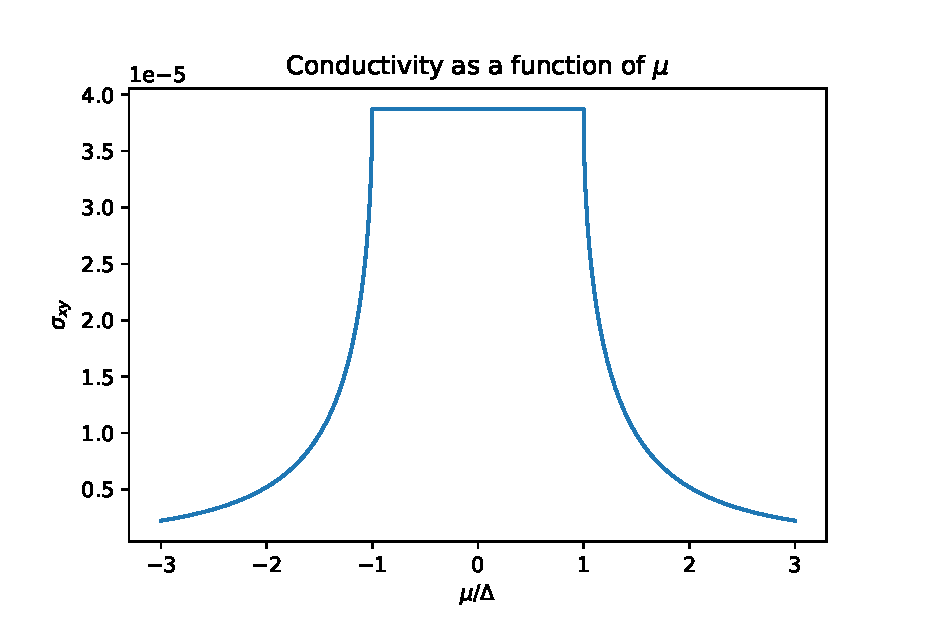
\includegraphics[width=\linewidth]{Immagini/ValleyHall/sigma_xy.eps}
    \caption{Here is shown $\sigma_{xy}(\mu)$ (eq. \ref{eq:valley-conductivity-2}). Notice how, when $\mu \in [-\Delta,\Delta]$ then $\sigma_{xy}=\frac {e^2}{2\pi \hbar}$}
    \label{fig:sigma_xy}
\end{figure}
To be fear we only calculated $\sigma_{xy}$ for the electrons in the valley $K_1$, the conductivity for the other valley is just $-\sigma_{xy}$. So, putting it all together, we have

\begin{equation}
    \sigma_{K_i,xy}(\mu)=(-1)^i\frac {e^2}{2\pi \hbar}\Bigg[\frac{\sqrt{\mu^2-\Delta^2}}{\mu} \theta(\mu^2-\Delta^2) - \theta(\mu-\Delta)\Bigg]
    \label{eq:valley-conductivity-complete}
\end{equation}
However in most cases it's safe to assume that the chemical potential is inside the energy gap, so equation \ref{eq:valley-conductivity-complete} becomes
\begin{equation}
    \sigma_{K_i,xy}=(-1)^{i+1}\frac {e^2}{2\pi \hbar}
\end{equation}



\section{Non-local Charge transport}
If we apply a voltage $V$ in two opposite points of a strip of a ohmic material of width $W$ and infinite lenght, and  we see a current that flows from one point to another figure \ref{fig:beconcini_strip}.\newline
\begin{figure}
    \centering
    \includegraphics[width=0.7\linewidth]{Immagini/ValleyHall/beconcini_strip.pdf}
    \caption{Representation of the strip}
    \label{fig:beconcini_strip}
\end{figure}
Clearly the current isn't completely localized along the axis that unites the two injection points, and so does the voltage difference.\newline
If we probe the voltage from two different points with an offset of $x$ from the injection points and we divide it by the total current between the contacts we see that  

\begin{equation}
    \frac{V(x)}I=\frac{2\rho}\pi\ln\bigg |\coth \Big(\frac{\pi x}{2W}\Big)\bigg |
\end{equation}
Where $\rho$ is the resistivity. Don't worry later on there is the proof of this equation.\newline

However, two-dimentional material like gapped graphene \cite{gorbachev2014detecting,sui2015gate,shimazaki2015generation} and transition metal dichalcogenides \cite{xiao2012coupled,mak2014valley,lee2017valley}, don't obey this equation. This is because theese materials display the Valley Hall effect we talked about previously (inserire reference a sezione).

Non-local transport can be a useful tool to probe the existance of anomalous Hall effect \cite{valenzuela2006direct,abanin2009nonlocal,brune2010evidence,abanin2011giant,balakrishnan2013g,wang2015proximity}


\section{Theory of non local charge transport}

The charges inside the material get pushed around from the electrochemical potential $\psi_K$


\begin{equation}
    \psi_{K}(\vect r)= V(\vect r)-\frac 1e \mu_K[n_{K_1}(\vect r),n_{K_2}(\vect r),T]
\end{equation}

Where $\phi$ is the electrical potential, and $\mu_K=\frac {\partial}{\partial n_{K}}F[n_{K_1}(\vect r),n_{K_2}(\vect r),T]$ is the chemical potential of the material and $F$ is the free energy.

The current generated from this potential in the valley $K_\alpha$ in the $i-$th direction is

\begin{equation}
    -eJ_{K_\alpha,i}(\vect r)= \sum_{j,b} \underbrace{-\sigma_{K_\alpha K_\beta ,ij}}_{\textrm{conductivity}}\partial_j\psi_{K_\beta }(\vect r)
\end{equation}
From now we are going to set $T\approx 0$\footnote{A more precise statement is that the thermal De Broglie wavelenght $\lambda_T$ must be much larger than the average distance between the electrons. We are not going into the math here, but if you want to calculate it, keep in mind that the dispersion relation is relativistic, so the formula of $\lambda_T$ is going to be a bit different}
and ignore intervalley scattering, so if $K_\alpha \neq K_\beta $ $\sigma_{K_\alpha K_\beta ,ij}=0$, also because of this the free energy can be written as the sum of the two Free energies
\begin{equation}
    F(n_{K_1},n_{K_2})=F_1(n_{K_1}(\mathbf r))+F_2(n_{K_2}(\mathbf r))
\end{equation}
And so the chemical potential of a given valley depend only on the number of electron in the same valley
\begin{equation}
    \mu_\alpha(n_{K_\alpha}(\mathbf r))=\frac{\partial}{\partial n_{K_\alpha}}F(n_{K_0},n_{K_1})=\frac{\partial}{\partial n_{K_\alpha}}F_\alpha(n_{K_\alpha}(\mathbf r))
\end{equation}
This simplifies the trasport equation in 

\begin{equation}
    -e\mathbf J_{K_{\alpha}}(\mathbf r)= \sigma_{K_\alpha}(\mathbf r)\nabla \psi_{K_\alpha}(\mathbf r)
    \label{eq:current-1}
\end{equation}
Where $\sigma_{K_\alpha}$ is the following matrix
\[
    \sigma_{K_\alpha}=
    \begin{bmatrix}
        \sigma_{K_\alpha K_\alpha,xx} & \sigma_{K_\alpha K_\alpha,xy}\\
        -\sigma_{K_\alpha K_\alpha,xy}^* & \sigma_{K_\alpha K_\alpha,xx}
    \end{bmatrix}
\]
Now we need to write the gradient electrochemical potential $\nabla \psi(\vect r)$
\begin{equation}
    \nabla \psi_{K_\alpha}(\mathbf r)=\nabla V(\mathbf r) -\frac 1e \frac{\partial}{\partial n_{K_\alpha}}\mu_\alpha(n_{K_\alpha}(\mathbf r))\nabla n_{K_\alpha}
    \label{eq:echemical1}
\end{equation}
From equation INSERIRE REFERENCE A EQUAZIONE we can write for gapped Dirac hamiltonians that VERIFICARE SE VALE ANCHE PER BILAYER GRAPHENE  \[\frac{\partial \mu_{K_\alpha}}{\partial n_{K_\alpha}}=\frac{\pi}{\sqrt{2\pi |n|+\Delta^2}}+\Delta\delta(n)\approx \frac \pi\Delta +\Delta\delta(n) \quad \forall \alpha\]
In this equation we assumed that there are very few charge carries, so $\frac n{\Delta^2}\approx 0$. We can shorten the equation \ref{eq:echemical1} by defining
\begin{equation}
    e^2D_{K_\alpha,ij}=\sigma_{K_\alpha, ij}\frac{\partial \mu_\alpha}{\partial n_{K_\alpha}}[n_{K_\alpha}(\mathbf r)]
\end{equation}
So equation \ref{eq:current-1} becomes

\begin{equation}
    -eJ_{K_\alpha,i}(\mathbf r)=\sigma_{K_\alpha, ij}E_j(\mathbf r) -eD_{K_\alpha,ij}\partial _jn_{K_\alpha}(\mathbf r)
\end{equation}
or, written in matrix form
\begin{equation}
    -e\mathbf J_{K_\alpha}(\mathbf r)=\sigma_{K_\alpha}\mathbf E(\mathbf r) -eD_{K_\alpha}\nabla n_{K_\alpha}(\mathbf r)
\end{equation}
Where $\sigma_{K_\alpha}$ and  $-eD_{K_\alpha}$ are matrices.

\subsection{Re-writing the equations in terms of charge current and valley current}
Measuring the currents in different valley can be cumbersome, however measuring the charge current $\mathbf J_{c}=\mathbf J_{K_1}+\mathbf J_{K_2}$ is straightforward, and for mathematical convenience we also define the valley current $\mathbf J_{v}=\mathbf J_{K_1}-\mathbf J_{K_2}$.

Since we no longer describe the currents in terms of their valley index, but on the sum and the difference of what happens at the different valleys, we are going to reparametrize also the other quantities in the same fashion.


\begin{equation}
    \begin{cases}
        \sigma_c=\sigma_{K_1}+\sigma_{K_2}=2\sigma_{xx}\delta_{ij}\\
        \sigma_v=\sigma_{K_1}-\sigma_{K_2}=\sigma_v=2\sigma_{xy}\epsilon_{ij}
    \end{cases}
\end{equation}
The term $-eD_{K_\alpha}\nabla n_{K_\alpha}(\mathbf r)$ is a little harder to traslate. First off we are going to impose the local charge conservation

\[
    n(\mathbf r)=n_{K_0}+n_{K_1}\approx 0
\]
and so 

\begin{equation}
    n_v(\mathbf r)=n_{K_1}-n_{K_2}=2n_{K_1}=-2n_{K_2}
\end{equation}
Now let's do the sum of the $D_{K_\alpha}\nabla n_{K_\alpha}(\mathbf r)$ terms to write them in terms of charge and valleys degrees of freedom

\[D_{K_1}\nabla n_{K_1}+D_{K_2}\nabla n_{K_2}=(D_{K_1}-D_{K_2})\nabla n_v(\mathbf r)/2\]

\[D_{K_1}-D_{K_2}=\sigma \frac{\partial \mu_1}{\partial n_{K_1}}- \sigma^T \frac{\partial \mu_2}{\partial n_{K_2}}\]
since $\mu_v=2\mu_1=-2\mu_2$ and $n_v=2n_{K_1}=-2n_{K_2}$

\[D_{K_1}-D_{K_2}=\frac 1{e^2}(\sigma-\sigma^T)\frac{\partial \mu_v}{\partial n_v}=\frac 2{e^2}\sigma_v\frac{\partial \mu_v}{\partial n_v}\]
so I define 

\[D_{cv}=\frac 2{e^2}\sigma_v\frac{\partial \mu_v}{\partial n_v}\approx\frac 2{e^2} \frac \pi\Delta\sigma_v\]
so we get that

\[D_{K_1}\nabla n_{K_1}+D_{K_2}\nabla n_{K_2}=D_{cv}n_v\]
Putting it all together we have that

\[\mathbf J_c(\mathbf r)=\sigma_c \mathbf E(\mathbf r)+eD_{cv}\nabla n_v(\mathbf r)\]
Writing all the indices

\[J_{c,i}=\sum_j \sigma_{c,xx}\delta_{ij}E_i+D_{cv,xy}\epsilon_{ij}\partial_j n_v\]
so we can rewrite them as

\[\mathbf J_{c}= \sigma_{c,xx}\mathbf E_i + D_{cv,xy} \nabla \times n_v\]
where $\sigma_{c,xx}$ and $D_{cv,xy}$ are scalars



	\chapter{Theory of the non-local resistance}
	Let's from the frequency response of the non-local response that we talked about in section \ref{sec:beconcini} \cite{Beconcini_2016}
\begin{equation}
    R_{\textrm{NL}}(k)=\frac{2\omega(k)}{k\sigma_c}
    \bigg\{
        \frac{\omega(k)}{\tanh(kW/2)} + \frac{k\tan^2(\theta_{\textrm{VH}})}{\tanh[\omega(k)W/2]}    
    \bigg\}^{-1}
    \label{eq:rnlk}
\end{equation}
Its anti-fourier transform tells us everything we would want to know about the system. Unfortunately \ref{eq:rnlk} doesn't have an analytic Fourier transform.\\ If there are no topological effect $\theta_{\textrm{VH}}=0$ and it can be solved analytically.
\begin{equation}
    R_{\textrm{NL}}(k)|_{\theta_{\textrm{VH}}=0}\equiv R_{\textrm{NL}}^{(0)}(k)=
    \frac{2\rho}k\tanh\bigg(\frac{kW}2\bigg)
    \label{eq:ohmick}
\end{equation}

\begin{equation}
    R_{\textrm{NL}}^{(0)}(x)=
    \mathcal F^{-1}\left[R_{\textrm{NL}}^{(0)}(k) \right]=
    -\frac{2\rho}\pi\ln\bigg |\tanh \Big(\frac{\pi x}{2W}\Big)\bigg |
    \label{eq:ohmic signal2}
\end{equation}
This is the purely ohmic nonlocal signal that we have talked about in \ref{eq:ohmic signal}.\\
However, if we are going to explore topological materials we cannot set $\tan (\theta_{\textrm{VH}})=0$, this means that we'll have to do some approximations.

\section{Study of $R_{\textrm{NL}}(x)$}

Let's look at the graph of the $R_{\textrm{NL}}(k)$ before doing any approximations:
\begin{figure}[h!]
    \centering
    \includegraphics[width=\linewidth]{Immagini/rnl/widths.pdf}
    \caption{$R_{NK}(k)$ for several values of $W/l_\textrm{v}$. The dashed black line represents where $k=1/l_\textrm{v}$, the colored dashed line represents where $k=1/W$}
    \label{fig:RNLk}
\end{figure}
As you can see from the figure \ref{fig:RNLk} 
\begin{itemize}
    \item If $W\gg l_\textrm{v}$ we have a single bell like function with the width of the bell being $\approx 1/W$ and the height being $R_{xx}$ 
    \item If $W\ll l_\textrm{v}$ we have a double-bell function, where the first bell has a height of $R_{xx}$ and a width of $\approx 1/l_\textrm{v}$, and the second one has a shorter height.
\end{itemize}    
To evaluate the precise height of the secondary bell we just need to set $l_\textrm{v}^{-1}\ll k \ll W^{-1}$ in equation \ref{eq:rnlk}, this gives us

\begin{equation}
    R_{\textrm{NL}}(l_\textrm{v}^{-1}\ll k \ll W^{-1})\approx R_{xx}\cos^2(\theta_{\textrm{VH}})   
    \label{eq:plateau} 
\end{equation}
Where $R_{xx}=\frac{W}{\sigma_{xx}}$ and $\cos^2(\theta_{\textrm{VH}})=\frac{1}{1+\tan^2(\theta_{\textrm{VH}})}$

So, if we have $l_\textrm{v}\ll W$ or $\theta_{\textrm{VH}}\ll 1$ (or both) we have a single bell structure. Incidentally these are the conditions to NOT have topological effects, so the less visible the double bell is, the less visible the topological effects are. We'll also see later how one of the bell represents the ohmic nonlocal signal, while the other represents the topological nonlocal signal. 

\subsection{Small $k$}
Let's start by exploring $k\ll l_\textrm{v}^{-1},W^{-1}$. This will tell us how the function behaves at long ranges $x\gg l_\textrm{v},W$. In this regime 

\begin{equation}
    \omega(k)=\sqrt{k^2+l_\textrm{v}^{-2}}\approx \frac 1{l_\textrm{v}}\left[1+\frac{(kl_\textrm{v})^2}2\right]
\end{equation}
\begin{equation}
    \coth (kW/2)\approx \frac 2{kW} + \frac{kW}6
\end{equation}
Plugging the last two equations into equation \ref{eq:rnlk} we have that $R_{\textrm{NL}}(k)\approx$
\begin{equation}
    \frac 2{\sigma_c}\frac 1 {l_\textrm{v}k}\left[
        \frac 1{l_\textrm{v}}\left(1+\frac{k^2l_\textrm{v}^2}{2}\right)\left(\frac 2{kW} + \frac{kW}6\right)+
        \frac{k\tan^2(\theta_{\textrm{VH}})}{\tanh(W/2l_\textrm{v})} + o(k^2)
    \right]^{-1}
\end{equation}
And after some steps we get that
\begin{equation}
    R_{\textrm{NL}}(k\ll l_\textrm{v}^{-1},W^{-1})=
    \frac {R_{xx}}{1+L_\textrm{v}^2k^2 + o(k^4)}
    \label{eq:lorentz0}
\end{equation}
Where the \textit{renormalized valley diffusion length} $L_\textrm{v}^2$ is defined as
\begin{equation}
    L_\textrm{v}^2 \equiv l_\textrm{v}^2+\frac {W^2}{12} +\frac{l_\textrm{v}W}2 \frac{\tan^2(\theta_{\textrm{VH}})}{\tanh(W/2l_\textrm{v})}
\end{equation}
Now we are going to define the topological nonlocal resistance $R_{\textrm{NL}}^T$ by taking the equation \ref{eq:lorentz0}, and ignoring the $o(k^4)$ term
\begin{equation}
    R_{\textrm{NL}}^T(k)\equiv
    \frac {R_{xx}}{1+L_\textrm{v}^2k^2}
    \label{eq:lorentz1}
\end{equation} 
We are now ready to do the Fourier transform of equation \ref{eq:lorentz1} to get the behavior for $x\gg l_\textrm{v},W$
\begin{equation}
    R_{\textrm{NL}}(x\gg l_\textrm{v},W)\approx\mathcal F^{-1}\left[R_{\textrm{NL}}^T(k)\right]\equiv R_{\textrm{NL}}^T(x)
\end{equation}
That is equal to 

\begin{equation}
    R_{\textrm{NL}}^T(x)=
    R_{xx}\int_{-\infty}^{+\infty}
    \frac {e^{-ikx}}{1+L_\textrm{v}^2k^2}
    \frac {dk}{2\pi}=
    \frac{R_{xx}}{2L_\textrm{v}}e^{-\frac{|x|}{L_\textrm{v}}}
\end{equation}
So,
\begin{equation}
    R_{\textrm{NL}}(x\gg l_\textrm{v},W)\approx R_{\textrm{NL}}^T(x)
    \label{eq:rxg}
\end{equation}

\subsection{Big $k$}
Fortunately the case for which $k\gg l_\textrm{v}^{-1}$ is much simpler: in this case $\omega(k) \approx k$, so

\begin{equation}
    R_{\textrm{NL}}(k\gg l_\textrm{v}^{-1})=\cos^2(\theta_{\textrm{VH}})\frac {2\rho}{k}\tanh\left(\frac{kW}2\right)
\end{equation}
Using equation \ref{eq:ohmick} we get that this last equation is $\cos^2(\theta_{\textrm{VH}})$ times the one for the purely ohmic nonlocal signal
\begin{equation}
    R_{\textrm{NL}}(k\gg l_\textrm{v}^{-1})\approx
    \cos^2(\theta_{\textrm{VH}})R_{\textrm{NL}}^{(0)}(k)
\end{equation}
This means that the Fourier transform is
\begin{equation}
    R_{\textrm{NL}}(x\ll l_\textrm{v})\approx\cos^2(\theta_{\textrm{VH}})R_{\textrm{NL}}^{(0)}(x)
    \label{eq:rxl}
\end{equation}
\subsection{Testing the approximations}
But how do these equations fear in practice?
\begin{figure}[h!]
    \centering
    \includegraphics[width=\linewidth]{Immagini/rnl/2approx.pdf}
    \caption{For this example $l_\textrm{v}=20W$}
    \label{fig:rnl2approx}
\end{figure}
As you can see from figure \ref{fig:rnl2approx} the two approximations work pretty well, except in the neighborhood where $k\approx l_\textrm{v}^{-1}$. But what we really care about is $R_{\textrm{NL}}(x)$.\\
If we plot the approximations for $x\gg l_\textrm{v},W$ (eq. \ref{eq:rxg}) and $x\ll l_\textrm{v}$ (eq. \ref{eq:rxl}) alongside the numerical Fourier transform of $R_{\textrm{NL}}(k)$ \ref{eq:rnlk} we get figure \ref{fig:rnlx2approx}

\begin{figure}[h!]
    \centering
    \includegraphics[width=\linewidth]{Immagini/rnl/x2approx.pdf}
    \caption{The parameters for this graph are exactly the same for the previous graph (figure \ref{fig:rnl2approx})}
    \label{fig:rnlx2approx}
\end{figure}
\subsection{Improving the approximation}
We can do better than this! By combining the two approximations it's possible to have a single equation that is very accurate for both $x\gg l_\textrm{v},W$ and $x\ll l_\textrm{v}$, however, in the end we'll end up with an approximation that is surprisingly good even for  $x\approx l_\textrm{v}$.

Since the Fourier transform is a linear operator, the idea is to find the linear combination of the two approximation that best approximates the $R_{\textrm{NL}}(k)$ for both $k\ll l_\textrm{v}^{-1},W^{-1}$ and $k\gg l_\textrm{v}^{-1}$ and then anti-transform the result.
\[
    R_{\textrm{NL}}(k)\approx \alpha R_{\textrm{NL}}(k\ll l_\textrm{v}^{-1},W^{-1}) +\beta R_{\textrm{NL}}(k\gg l_\textrm{v}^{-1})=
\]
\[
    =R_{\textrm{NL}}(k)\approx \alpha R_{\textrm{NL}}^T(k) +\beta\cos^2(\theta_{\textrm{VH}}) R_{\textrm{NL}}^{(0)}(k)      
\]
Where $\alpha$ and $\beta$ are the coefficient to be determined.\\
Since we only need to evaluate two variables, we only need to evaluate the expression above in two different points. The most reasonable points to choose are $k=0$ and $k=+\infty$, since they are the points where the approximations work better. For doing the calculations it's best to write out the two approximations 
\[
    R_{\textrm{NL}}(k)\approx 
    \alpha \frac {R_{xx}}{1+L_\textrm{v}^2k^2}+
    \beta\frac {2\rho}{k}\tanh\left(\frac{kW}2\right)\cos^2(\theta_{\textrm{VH}})
\]
\begin{itemize}
    \item For $k\to +\infty$ the term that is multiplied by $\beta$ is an increasingly precise estimate of $R_{\textrm{NL}}(k)$, and it dominates over the term that is multiplied by alpha, so $\beta=1$.
    \item For $k=0$ we have that
    \[
        R_{xx}=\alpha R_{xx} +  R_{xx}\cos^2(\theta_{\textrm{VH}})   
    \]
    So, $\alpha=\sin^2(\theta_{\textrm{VH}})$. 
\end{itemize}
Putting it all together we define the resulting approximation
\begin{equation}
    \boxed{
        \tilde R_{\textrm{NL}}(k)\equiv
        \sin^2(\theta_{\textrm{VH}})R_{\textrm{NL}}^{T}(k)+
        \cos^2(\theta_{\textrm{VH}})R_{\textrm{NL}}^{(0)}(k)
    }
\end{equation}
The thing that I personally like about this approximation is its geometrical elegance. If we write all the terms of the equation above we get
\begin{equation}
    \tilde R_{\textrm{NL}}(k)\equiv
    \sin^2(\theta_{\textrm{VH}})\frac {R_{xx}}{1+L_\textrm{v}^2k^2}+
    \cos^2(\theta_{\textrm{VH}})\frac {2\rho}{k}\tanh\left(\frac{kW}2\right)
\end{equation}
And if we plot the approximation $\tilde R_{\textrm{NL}}(k)$ alongside the actual values of $R_{\textrm{NL}}(k)$ we can see that they are remarkably similar (figure \ref{fig:kapproxcomp})
\begin{figure}[h!]
    \centering
    \includegraphics[width=\linewidth]{Immagini/rnl/kapproxcomp.pdf}
    \caption{Comparison between $R_{\textrm{NL}}(k)$ and $\tilde R_{\textrm{NL}}(k)$. The continuous line represents $R_{\textrm{NL}}(k)$, while the dashed line represents $\tilde R_{\textrm{NL}}(k)$. It's unreasonably accurate!}
    \label{fig:kapproxcomp}
\end{figure}\\
The nice thing about this is that if two equations are similar, then their Fourier transform will be too.
This means that $\tilde R_{\textrm{NL}}(x)$ will be a good approximation of $R_{\textrm{NL}}(x)$, where
\begin{equation}
    \boxed{
        \tilde R_{\textrm{NL}}(x)=
        \sin^2(\theta_{\textrm{VH}})R_{\textrm{NL}}^T(x)+
        \cos^2(\theta_{\textrm{VH}})R_{\textrm{NL}}^{(0)}(x)
    }
    \label{eq:rnl}
\end{equation}
We can write out the full formula using equations \ref{eq:rxg} and \ref{eq:rxl}
\begin{equation}
    \tilde R_{\textrm{NL}}(x)=
    \frac{R_{xx}}{2L_\textrm{v}}e^{-|x|/L_\textrm{v}}\sin^2(\theta_{\textrm{VH}})-
    \frac{2R_{xx}}{\pi W}\ln \bigg|\tanh \Big(\frac{\pi x}{2W}\Big)\bigg|\cos^2(\theta_{\textrm{VH}})
\end{equation}
Infact if we re-create figure \ref{fig:rnlx2approx} with the equation above we get figure \ref{fig:rnlxapprox}
\begin{figure}[h!]
    \centering
    \includegraphics[width=\linewidth]{Immagini/rnl/xapprox.pdf}
    \caption{As you can see it's impossible to distinguish the difference between the two functions to the naked eye. The parameters are the same as figure \ref{fig:rnlxapprox}}
    \label{fig:rnlxapprox}
\end{figure}
	\section{$R_{NL}(x)$ as we change $\rho_{xx}$}
Hall effect experiments are generally done in the so-called Hall-bars. There are samples of material with a shape like the one in figure \ref{fig:hall-bar}. This also means that more often than not in experimental setups we cannot change $x$ without changing the geometry of the sample.
\begin{figure}[h!]
    \centering
    \includegraphics[width=\linewidth]{Immagini/rnl/hallbarbrutta.png}
    \caption{Example of the experimental setup}
    \label{fig:hall-bar}
\end{figure}\\
In the previous section we studied how $R_{NL}$ depended on $x$, and Hall-bars can only measure a single $x$. One way for having multiple measuraments with the same Hall-bar is to change the resistivity of the material by changing the temperature of the setup, and study $R_{NL}$ as we change $\rho_{xx}$.

For convenience let's re-write equation \ref{eq:rnlk}
\[
    R_{NL}(k)=\frac{2\omega(k)}{k\sigma_c}
    \bigg\{
        \frac{\omega(k)}{\tanh(kW/2)} + \frac{k\tan^2(\theta_{VH})}{\tanh[\omega(k)W/2]}    
    \bigg\}^{-1}
\]
For convenience, we are going to change $\tan(\theta_{VH})=\sigma_v\rho_{xx}$ and do a taylor series expansion of the above equation around $\tan^2(\theta_{VH})\approx 0$.

\[
    R_{NL}(k)\approx R_{NL}(k)|_{\tan^2(\theta_{VH})=0} +
    \frac \partial {\partial \tan^2(\theta_{VH})} R_{NL}(k)|_{\tan^2(\theta_{VH})=0}
\]
that we are going to re-define as
\[
    R_{NL}(k)\approx R_{NL}^{(0)}(k) + R_{NL}^{(1)}(k)
\]
The zeroth order term gives us this:
\[
    R_{NL}^{(0)}(k)=\frac{2\rho}k\tanh\bigg(\frac{kW}2\bigg)
\]
And if we do a the Fourier transform to get the $x$ dependent form we get the ohmic nonlocal resistivity \ref{eq:ohmic signal}
\begin{equation}
    R_{NL}^{(0)}(x)=\frac{2\rho}\pi\ln\bigg |\coth \Big(\frac{\pi x}{2W}\Big)\bigg |
\end{equation}
Now let's calculate the first order term

\[
    R_{NL}^{(1)}(k)=-2\rho\frac{\omega(k)}k\bigg[\frac{\omega(k)}{\tanh(Wk/2)} \bigg]^{-2}k\frac{\tan^2(\theta_{VH})}{\tanh(\omega(k)W/2)}=
\]
\[
    =-2\rho^3\sigma_v^2 \tanh^2\bigg(\frac{kW}2\bigg)\bigg\{\omega(k)\tanh\bigg[\frac{\omega(k) W}2\bigg]\bigg\}^{-1}\equiv
    \rho^3F(k)
\]
where $F(k)$ is defined as follows

\begin{equation}
    F(k)\equiv -2\sigma_v^2\tanh^2\bigg(\frac{kW}2\bigg)\bigg\{\omega(k)\tanh\bigg[\frac{\omega(k) W}2\bigg]\bigg\}^{-1}
\end{equation}
And it doesn't depend on $\rho$

Putting it all together we get that

\begin{equation}
    \lim_{\rho\to 0} R_{NL}(x)= \frac{2\rho}\pi\ln\bigg |\coth \Big(\frac{\pi x}{2W}\Big)\bigg | + \rho^3F(x) + o(\rho^5)
\end{equation}

PARLARE DEI REGIMI IN CUI DOMINA $\rho^3$

Now let's study what happens when $\rho,\tan(\theta_{VH})\to \infty$. First off let's rewrite equation \ref{eq:rnlk} and bring the $\omega(k)$ and $k$ inside the curly braces.

\[
    R_{NL}(k)=2\rho
    \bigg\{
        \underbrace{\frac{k}{\tanh(kW/2)}}_{\substack{\text{cannot be}\\\text{ignored for } k=0}} + \frac {k^2}{\omega(k)}\frac{\tan^2(\theta_{VH})}{\tanh[\omega(k)W/2]}    
    \bigg\}^{-1}
\]

This limit is a bit tricky to evaluate. First off even thought the right-most term inside the curly braces dominates everywhere except for $k=0$ this "\emph{small detail}" is crucial. From image \ref{fig:rho1} we can see that the larger $\rho$ gets, the smaller the area around $k=0$ where the first term dominates.
\begin{figure}[h!]
    \centering
    \includegraphics[width=\linewidth]{Immagini/rnl/rho1.pdf}
    \caption{The continuous blue line represents the first term, the blue dashed line represents its approximation around $k=0$ and the gray dashed lines represent its approximation for $k\to \infty$.\newline The orange parabola represents the right-hand side term $\frac {k^2}{\omega(k)}\frac{\tan^2(\theta_{VH})}{\tanh[\omega(k)W/2]}$}
    \label{fig:rho1}
\end{figure}\\
For high values of $\rho, \tan(\theta_{VH})$ the parabola becomes really narrow and it overtakes the first term with $k\approx 0$. This means that we can approximate the first term as being always equal to $2/W$. This means that
\begin{equation}
    \lim_{\rho\to\infty} R_{NL}(k)=2\rho
    \bigg\{
        \frac 2W+ \frac {k^2}{\omega(k)}\frac{\tan^2(\theta_{VH})}{\tanh[\omega(k)W/2]}    
    \bigg\}^{-1}
\end{equation}



	\section{Comparison with experimental data}
Experimental setups have a few limitations compared to the theoretical treatment, for example you do not have complete freedom of changing the resistance, rather the resistance is changed by changing the temperature of the sample.
This has a few consequences: 
\begin{itemize}
    \item Since out sample is a semiconductor, the lower the temperature, the higher the resistance, but if the temperature gets too low we enter the ballistic regime, and our treatment is no longer valid.
    \item If the temperature gets too high, the quantization of the hall effect disappears
\end{itemize}
This restricts us to a couple order of magnitude of the resistivity.

Now we compare the results with the experimental data. Let's start from analyzing the data from  \cite{rebecca2022moirè}.\\
In this paper the authors measured the valley hall effect of a heterostructure made of bilayer-graphene on top of boron nitride at different angles $\phi$ between the graphene and the boron nitride. The sample has a width $W=1.7\mu$m, and inter-valley scattering length $l_{\textrm v}=1.6\mu$m and the distance of the contact from the injection point is $x=2.3\mu$m

The angles $\phi$ that were explored are $0,\pi/6$ and $\pi/3$. If you plot the measurements you get figure \ref{fig:rebeccadatapoints}.\\
\begin{figure}[h!]
    \centering
    \includegraphics[width=\linewidth]{Immagini/rnl/rebecca_data.pdf}
    \caption{Datapoints from \cite{rebecca2022moirè}}
    \label{fig:rebeccadatapoints}
\end{figure}
We then analyze the data by comparing the output of the model thus far developed to the data, we did not fit the data, rather we used the knowledge we already have about the parameters $W,l_\textrm{v},x$ and plot the result on top of the datapoints.
\begin{itemize}
    \item For $\phi=\pi/3$ we have that the response is fully ohmic, and so we get a completely linear response (figure \ref{fig:rebecca pi/3})
    \item For $\phi=\pi/6$ we have a hall effect, however, since $W\approx l_\textrm{v}$ the ohmic and the topological response mix together, so we never see the full-fledged $\rho^3$ behavior.\footnote{A more detailed explanation was given in the details of subsection \ref{sec:alternaterho}}
    \item For $\phi=0$ the response does not match the model we developed, further investigations should be done to address the discrepancy
\end{itemize}
\begin{figure}[h!]
    \centering
    \includegraphics[width=\linewidth]{Immagini/rnl/rebecca_0.pdf}
    \caption{Comparison between the data points and the theoretical expectation for $\phi=\pi/3$. With the exception of the last experimental point, the data follows the theoretical prediction}
    \label{fig:rebecca pi/3}
\end{figure}
\begin{figure}[h!]
    \centering
    \includegraphics[width=\linewidth]{Immagini/rnl/rebecca_1.pdf}
    \caption{Comparison between the data points and the theoretical expectation for $\phi=\pi/6$. The model has a lower precision for higher values of $\rho,R_{\textrm{NL}}$, however we can say that the data follow the theoretical prediction}
    \label{fig:rebecca pi/6}
\end{figure}
\begin{figure}[h!]
    \centering
    \includegraphics[width=\linewidth]{Immagini/rnl/rebecca_2.pdf}
    \caption{Comparison between the data points and the theoretical expectation for $\phi=0$. The model does not satisfactorily reflect the data.}
    \label{fig:rebecca 0}
\end{figure}

\section{Conclusions}
In this thesis we provided a complete and accurate description on the Nonlocal resistance arising from valley-Hall. It expands on top of the work done by Beconcini et al. \cite{Beconcini_2016} where they manage to explain the results Shimazaki et al. obtained  \cite{shimazaki2015generation} where they found a that the non-linear resistance on bilayer graphene depended on the cube of the longitudinal resistivity ($R_\textrm{NL}\propto \rho^3$) for low resistivities and then it saturates.\\ 
The work done by Beconcini et al. was only able to explain the behavior of the nonlocal resistance if the width of the material is much smaller than the valley diffusion length ($l_v\ll W$). In this thesis we found an accurate description for any valley diffusion length and width and we compared the results with the work done by Arrighi et al. \cite{rebecca2022moirè}.
The results we obtained can also be used to study the non-local resistance of other anomalous Hall effect such as spin-Hall effect.

	
	
	
	\printbibliography

\end{document}